\documentclass[12pt,a4paper]{report}

% -------------------------
% PACKAGES
% -------------------------
\usepackage[utf8]{inputenc}
\usepackage[T1]{fontenc}
\usepackage[french]{babel}
\usepackage{lmodern}
\usepackage{geometry}
\usepackage{setspace}
\usepackage{amsmath,amssymb}
\usepackage{hyperref}
\usepackage{graphicx}
\usepackage{float}
\usepackage{placeins}
\usepackage{tikz}
%\usepackage{emoji}
\geometry{margin=2.5cm}
\onehalfspacing

% Hyperref
\hypersetup{
    colorlinks=true,
    linkcolor=blue,
    urlcolor=blue,
    citecolor=blue
}



% -------------------------
% PAGE DE GARDE (À PERSONNALISER)
% -------------------------
\begin{document}
\begin{titlepage}
    \centering
    {\Large \textbf{Université / Établissement}}\\[0.5cm]
    {\Large \textbf{Master ...}}\\[2cm]

    {\Huge \textbf{Titre du Mémoire}}\\[1cm]
    {\Large Basé sur l’article :}\\
    {\large \textit{Évaluation de l’efficacité numérique de la méthode IB–LB pour la modélisation tridimensionnelle à l’échelle des pores des écoulements et du transport.}}\\[2cm]

    \vfill

    \begin{flushleft}
    \textbf{Étudiant :} Nom Prénom \\
    \textbf{Encadrant(s) :} Nom Prénom \\
    \textbf{Année universitaire :} 2024–2025
    \end{flushleft}
\end{titlepage}

% -------------------------
% TABLE DES MATIÈRES
% -------------------------

\tableofcontents
\newpage

% -------------------------
% INTRODUCTION
% -------------------------

\chapter{Introduction générale}
\section{Contexte scientifique}
L’évolution temporelle des milieux poreux est influencée par des processus physico-chimiques, tels que l’altération ou la précipitation de phases minérales dans les roches, ainsi que par des activités biologiques, comme la croissance de biofilms bactériens ou l’obstruction biologique des pores. Ces transformations modifient directement les propriétés effectives du milieu, notamment la perméabilité et la surface spécifique.

Ces phénomènes jouent un rôle crucial dans de nombreuses applications souterraines : stockage de gaz (Kang et al., 2010 ; Ebigbo et al., 2013), formation de gisements miniers (Zhao et al., 2014), biorémédiation in situ (Thullner et al., 2002), lessivage ou extraction de sel (Luo et al., 2014). L’importance de ces applications a suscité un intérêt croissant pour la modélisation précise des écoulements et du transport dans des milieux poreux évolutifs.

Traditionnellement, les modèles se concentraient sur le comportement macroscopique des milieux poreux, où la loi de Darcy reste applicable. Cependant, les variations locales de la géométrie des pores, telles que leur obstruction ou leur élargissement, conduisent à une canalisation du flux et à une complexification progressive des phénomènes de transport. La compréhension détaillée de ces interactions nécessite des simulations à l’échelle des pores, rendues possibles grâce aux avancées récentes en ressources de calcul et aux méthodes numériques efficaces, notamment la méthode de Boltzmann sur réseau (LBM).

La LBM est particulièrement adaptée aux géométries complexes et à la parallélisation des algorithmes. Toutefois, sa nature cartésienne la rend moins adaptée aux géométries évolutives. Pour pallier cette limitation, plusieurs techniques numériques ont été développées, regroupées en méthodes conformes et non conformes aux frontières.
\section{Problématique}
Les méthodes conformes, comme l’approche Lagrangienne–Eulérienne arbitraire (ALE), maintiennent le maillage aligné avec les frontières physiques. Elles sont efficaces pour des interactions fluide–structure simples, mais deviennent coûteuses en 3D ou dans le cas de géométries complexes, et peuvent réduire la précision des schémas numériques.

Les méthodes non conformes, telles que la méthode du volume de fluide (VOF), la méthode Level-Set, le suivi de front ou la méthode de suivi de volume, permettent de gérer des interfaces mobiles plus flexiblement, mais la reconstruction de l’interface peut être numériquement coûteuse.

Dans ce contexte, les méthodes cartésiennes de type Immersed Boundary Method (IBM) apparaissent comme une alternative prometteuse pour traiter les interactions fluide–structure. Elles permettent de résoudre les équations de Navier–Stokes sur un maillage fixe non conforme, en immergeant les frontières dans la grille et en modifiant localement les équations à l’aide d’un terme de forçage.

Le couplage IBM–LBM s’avère particulièrement pertinent pour la modélisation de géométries complexes et évolutives à l’échelle des pores. Cependant, très peu d’études ont simultanément considéré l’écoulement et le transport en présence d’interfaces mobiles dans ce cadre, ce qui constitue la problématique centrale de ce travail.
\section{Objectifs du mémoire}
L’objectif principal de ce mémoire est d’examiner le potentiel de la méthode IBM pour la modélisation couplée de l’écoulement fluide et du transport de soluté dans des milieux poreux évoluant dans le temps.

Les objectifs spécifiques sont les suivants :

	1.	Étudier l’impact de l’évolution géométrique des pores, notamment le colmatage progressif, sur les propriétés hydrodynamiques et le transport des espèces chimiques.
    
	2.	Évaluer la précision des simulations IB–LBM en fonction de la dégradation du maillage liée à la complexité des interfaces.
    
	3.	Comparer différentes stratégies de forçage (direct, rétroactif, interpolé) pour les simulations IBM–LBM et identifier les conditions optimales d’application.
    
	4.	Proposer une approche quasi-stationnaire, consistant à simuler différentes géométries fixes successives, représentatives des phases d’évolution temporelle du milieu poreux.
    


\section{Organisation du mémoire}
La mémoire est structurée comme suit :

	•	Chapitre 1 : Introduction générale 
    – Présentation du contexte scientifique, de la problématique, et des objectifs.
    
	•	Chapitre 2 : Revue bibliographique 
    – Description des méthodes numériques existantes (LBM, IBM, ALE, Level-Set, VOF), de leurs avantages et limites, et analyse des travaux précédents.
    
	•	Chapitre 3 : Méthodologie 
    – Présentation de la méthodologie adoptée pour les simulations IB–LBM, génération des géométries poreuses et protocoles de simulation.
    
	•	Chapitre 4 : Résultats et discussion
    – Analyse des résultats numériques, évaluation de l’impact de l’évolution des pores sur l’écoulement et le transport.
    
	•	Chapitre 5 : Conclusion et perspectives
    – Synthèse des contributions, limites de l’étude et suggestions pour des travaux futurs.
    
% -------------------------
% CHAPITRE 2 — ÉTAT DE L’ART
% -------------------------

\chapter{Revue bibliographique}

\section{Modélisation des écoulements aux petites échelles}
Méthodes classiques (Navier–Stokes, éléments finis, ALE, etc.).
L’étude des écoulements dans les milieux continus repose historiquement sur les équations de Navier–Stokes, qui décrivent la conservation de la masse, de la quantité de mouvement et, le cas échéant, de l’énergie. Ces équations constituent la base de la mécanique des fluides classique et permettent de modéliser une large gamme de phénomènes, allant des écoulements laminaires simples jusqu’aux phénomènes turbulents plus complexes. Leur résolution analytique étant limitée à des géométries très idéalisées, le recours à des méthodes numériques s’est imposé comme une approche incontournable.

Parmi ces méthodes numériques, la méthode des éléments finis (FEM) occupe une place centrale. Elle consiste à discrétiser le domaine physique en un maillage composé d’éléments (triangles, quadrilatères, tétraèdres, etc.) sur lesquels les équations gouvernantes sont approximées à l’aide de fonctions de forme. La FEM offre une grande flexibilité pour traiter des géométries complexes et des conditions aux limites variées, ce qui en fait l’une des approches les plus utilisées pour la modélisation des écoulements en milieux poreux ou en domaines déformables.

Toutefois, lorsque les frontières du domaine évoluent au cours du temps — par exemple en présence de déformations de la matrice solide, de croissance de dépôts, ou d’interfaces mobiles — la méthode ALE (Arbitrary Lagrangian–Eulerian) est souvent adoptée. Cette formulation combine les avantages des descriptions lagrangienne et eulérienne : le maillage peut suivre partiellement le mouvement de la frontière tout en conservant une qualité satisfaisante au sein du domaine. La méthode ALE permet ainsi d’améliorer la précision des simulations en limitant la distorsion du maillage, tout en restant compatible avec les équations classiques de Navier–Stokes.

Malgré leur robustesse et leur maturité, ces approches traditionnelles présentent certaines limites lorsqu’il s’agit de simuler des dynamiques d’interface fortement non linéaires, des géométries très complexes ou des problématiques multiphysiques à l’échelle du pore. Ces défis ont conduit au développement de méthodes alternatives plus adaptées, telles que la méthode de Boltzmann sur réseau (LBM) et les méthodes de frontière immergée, qui permettent de traiter plus efficacement les interfaces complexes et les évolutions géométriques.
\section{Méthode Lattice Boltzmann (LBM)}
Principe, avantages, limites.
1. Principe de la LBM

La méthode de Boltzmann sur réseau (Lattice Boltzmann Method, LBM) est une approche numérique fondée sur la mécanique statistique.
Elle modélise l’écoulement fluide en suivant l’évolution d’une distribution de particules fictives se déplaçant et entrant en collision sur un réseau cartésien discret.

Le principe repose sur trois idées majeures :

(a) Discrétisation mésoscopique

Au lieu de résoudre directement les équations de Navier–Stokes, la LBM résout une équation de Boltzmann discrète.
Cette équation décrit l’évolution des fonctions de distribution $f_k$, correspondant aux populations de particules dans différentes directions $e_k$.

(b) Deux étapes fondamentales

À chaque pas de temps, deux opérations sont effectuées :
	1.	Collision
Les distributions $f_k$ relaxent vers un équilibre local $f_k^{(eq)} $selon le modèle BGK (temps de relaxation unique) ou MRT (temps multiples).
	2.	Propagation (streaming)
Les distributions résultantes sont transportées vers les nœuds voisins du réseau.

(c) Reconstruction des grandeurs macroscopiques

La vitesse du fluide, la densité et la pression sont calculées à partir des moments des fonctions $f_k$.

Cette approche permet de reproduire fidèlement les équations de Navier–Stokes dans le régime incompressible.



2. Avantages de la LBM

La LBM est devenue très populaire pour la simulation des écoulements en milieux complexes, notamment poreux, grâce à plusieurs avantages marquants :

 Adaptée aux géométries complexes

Les réseaux cartésiens simplifient la gestion :
	•	des milieux poreux,
	•	des interfaces tortueuses,
	•	des géométries obtenues par tomographie 3D.

Elle évite la génération de maillages non structurés coûteux.

Haut niveau de parallélisation

Les opérations locales de collision et propagation rendent la LBM :
	•	extrêmement adaptée au calcul parallèle (GPU, HPC),
	•	plus rapide que les méthodes Navier–Stokes classiques dans de nombreux cas.

 Simplicité d’implémentation

Les algorithmes de base sont faciles à coder et nécessitent peu d’opérations à chaque pas de temps.

 Bonne stabilité pour les écoulements de Stokes (Re bas)

Elle est particulièrement efficace pour les écoulements lents, très présents dans :
	•	les milieux poreux naturels,
	•	les systèmes microfluidiques.

 Couplage naturel avec les méthodes de frontière immergée (IBM)

Comme LBM et IBM utilisent des grilles cartésiennes, leur couplage (IB–LBM) permet :
	•	de traiter des interfaces mobiles,
	•	de suivre l’évolution géométrique des pores,
	•	d’obtenir de bonnes précisions même avec des maillages relativement grossiers.



3. Limites de la LBM

Malgré ses atouts, la LBM présente également plusieurs limites à prendre en compte.

 Maillage cartésien obligatoire

La LBM impose un maillage structuré, ce qui peut être contraignant pour :
	•	les corps de forme très irrégulière,
	•	les domaines non alignés avec la grille.

 Problèmes de compressibilité artificielle

Dans les formulations classiques :
	•	le fluide doit rester faiblement compressible,
	•	la vitesse doit être bien inférieure à la vitesse du son du modèle numérique.

Cela peut limiter certains régimes d’écoulement.

Sensibilité aux conditions aux limites

Les schémas bounce-back classiques :
	•	perdent en précision lorsque la frontière ne coïncide pas avec la grille,
	•	introduisent parfois des erreurs significatives dans les pores étroits.

C’est l’une des raisons pour lesquelles on utilise les méthodes IBM ou les bounce-back interpolés.

 Difficulté pour les écoulements turbulents

Bien que des versions existent (LES–LBM, MRT–LBM), la LBM :
	•	devient instable dans les régimes de Reynolds élevés,
	•	nécessite des modèles plus sophistiqués donc plus coûteux.

 Coût mémoire

Les réseaux (ex. D3Q19) stockent plusieurs distributions par nœud :
	•	ce qui augmente le coût mémoire comparé aux solveurs Navier–Stokes classiques,
	•	surtout en 3D.


\section{Méthode Immersed Boundary (IBM)}

La méthode de la frontière immergée (Immersed Boundary Method, IBM) a été introduite pour la première fois par Peskin (1972), dans le contexte de la modélisation de l’écoulement sanguin à l’intérieur du cœur. L’objectif initial était de représenter des structures souples, complexes et en mouvement sans recourir à un maillage conforme aux frontières. Depuis ces travaux pionniers, l’IBM a connu un développement important et s’est imposée comme une classe de méthodes numérique majeures pour la simulation des interactions fluide-structure. Des revues détaillées proposées notamment par Mittal ,Iaccarino (2005) et Sotiropoulos ,Yang (2014) ont permis de clarifier les nombreuses variantes de cette approche et leurs domaines d’applications.

D’un point de vue conceptuel, l’IBM repose sur une idée simple : les équations du fluide sont résolues sur une grille cartésienne fixe, tandis que les frontières solides (rigides ou déformables) sont représentées par des marqueurs immergés dans cette grille. Comme les frontières ne coïncident pas nécessairement avec les nœuds, un mécanisme de correction est nécessaire pour imposer les conditions de non-glissement ou de mouvement. Ce mécanisme dépend du type d’IBM considéré.



Approches sharp-interface et diffuse-interface

Les méthodes IBM se divisent généralement en deux grandes familles :

1) Approches “sharp-interface” (interface nette)

Ces approches visent à imposer la condition de frontière de manière localisée et précise, de sorte que l’interface demeure fine et bien définie.
Elles reposent typiquement sur :
	•	l’ajout d’un terme de forçage direct (direct-forcing method),
	•	des méthodes de cellules découpées (cut-cell),
	•	ou encore des corrections explicites des vitesses à proximité de l’interface.

Ces méthodes préservent une interface stricte et offrent une bonne précision géométrique, mais elles sont parfois sensibles aux oscillations numériques si le forçage n’est pas traité avec soin.

2) Approches “diffuse-interface”

Dans ces approches, l’interface fluide-solide est lissée sur quelques mailles et représentée au moyen :
	•	d’une force de pénalisation distribuée,
	•	d’un champ régulier de transition entre fluide et solide,
	•	ou de fonctions régulières (delta regularisé).

Elles sont plus robustes numériquement, mais introduisent un élargissement artificiel de la frontière, pouvant conduire à une perte locale de précision.


Intérêt de l’IBM pour la simulation à l’échelle des pores

La simulation pore-échelle présente des défis majeurs liés :
	•	à la géométrie extrêmement complexe,
	•	à la présence d’interfaces irrégulières,
	•	à l’évolution temporelle des parois (précipitation, dissolution, bio-obstruction),
	•	et à la nécessité de résoudre l’écoulement et/ou le transport dans des domaines tridimensionnels.

Dans ce contexte, l’IBM présente plusieurs avantages décisifs :

 1. Évite le maillage conforme aux frontières

La reconstruction du maillage en 3D est coûteuse, surtout lorsque les pores évoluent dans le temps.
L’IBM permet de garder une grille cartésienne fixe, réduisant considérablement :
	•	le coût numérique,
	•	la complexité de la génération du maillage,
	•	et les erreurs liées au remaillage.

 2. Gestion simple des géométries évolutives

Grâce à l’utilisation de marqueurs immergés, l’évolution de la géométrie (par exemple réduction de la gorge du pore) ne nécessite aucune régénération du maillage.

 3. Très bon couplage avec la méthode LBM

Les deux méthodes reposent sur des maillages cartésiens.
Le couplage IB–LBM :
	•	facilite l’imposition des conditions de non-glissement sur des interfaces complexes,
	•	améliore la précision en présence de pores très étroits,
	•	permet des simulations efficaces à maillage relativement grossier,
	•	et s’adapte naturellement aux changements géométriques.

 4. Bon compromis entre précision et coût de calcul

Les versions sharp-interface (ex. direct forcing) offrent une précision comparable à des schémas adaptés au maillage conforme, sans la complexité algorithmique associée.

\section{Méthodes de transport réactif}
Méthodes de transport réactif : approches VOF, reconstruction d’interface et schémas aux volumes finis (FVM)

La modélisation du transport réactif à l’échelle des pores pose plusieurs défis, en raison de la présence d’interfaces complexes, pouvant être réactives, mobiles ou partiellement perméables. La capacité à représenter correctement les flux diffusifs et advectifs à l’interface fluide–solide, ainsi qu’à capturer les gradients de concentration, est déterminante pour la fiabilité des simulations. Différentes approches numériques ont été développées pour traiter ces phénomènes, parmi lesquelles les méthodes VOF, les méthodes de reconstruction d’interface et les schémas aux volumes finis (FVM).



1. Approche Volume of Fluid (VOF)

L’approche VOF (Volume of Fluid), introduite par Hirt et Nichols (1981), est une méthode de suivi d’interface largement utilisée pour les écoulements diphasiques. Elle repose sur l’utilisation d’une fraction volumique (souvent notée $\phi$) permettant d’indiquer, pour chaque cellule du maillage, la proportion de fluide appartenant à une phase donnée.

Principe
	•	L’interface fluide/solide est représentée implicitement par une fonction indicatrice.
	•	Les équations de transport sont écrites sous une forme homogénéisée, c’est-à-dire valable dans toutes les cellules du maillage.
	•	Les propriétés locales (diffusion, vitesse, réaction) sont interpolées à partir des fractions volumiques.

Avantages
	•	Très simple à implémenter dans un schéma aux volumes finis.
	•	Aucune reconstruction géométrique explicite : l’interface est décrite implicitement.
	•	Convient lorsque les gradients de concentration sont faibles (hypothèse d’équilibre local).

Limites
	•	Peu précise lorsque les interfaces deviennent fines ou fortement réactives.
	•	Réduit la finesse de la description de l’interface → difficulté pour capturer les flux interfacials.
	•	Pas adaptée lorsque le nombre de Damköhler est élevé ou lorsque la cinétique de réaction est rapide.



2. Méthodes de reconstruction d’interface

Les méthodes de reconstruction d’interface offrent une alternative plus précise aux schémas VOF.
Elles reposent sur une description géométrique explicite de l’interface, souvent sous forme d’un plan local dans chaque cellule coupée.

Principe
	•	L’interface est reconstruite à partir de :
	•	marqueurs géométriques,
	•	champs de niveau (level-set),
	•	ou fraction volumique (VOF reconstruit).
	•	Les flux diffusifs et advectifs sont intégrés morceau par morceau, de part et d’autre de l’interface.
	•	La continuité des flux (conditions de transmission) est imposée explicitement.

Avantages
	•	Grande précision pour les flux interfacials, même avec forte discontinuité de propriétés.
	•	Adaptée au transport réactif avec réaction hétérogène à l’interface.
	•	Indispensable lorsque les gradients sont élevés (Da grand).

Limites
	•	Reconstruction géométrique potentiellement coûteuse, surtout en 3D.
	•	Complexité algorithmique plus élevée.
	•	Sensible à la qualité du maillage et à la courbure de l’interface.




3. Approches aux volumes finis (FVM)

Les schémas FVM constituent le cadre numérique le plus utilisé dans les simulations pore-échelle.
Ils permettent de résoudre les équations de transport :

$\nabla\cdot (u c) = \nabla\cdot(D \nabla c) - R(c)$

sur un maillage cartésien, conforme à celui utilisé par la LBM pour la résolution de l’écoulement.

Principe
	•	Les équations de transport sont intégrées dans chaque cellule.
	•	Les flux aux faces sont calculés par :
	•	interpolation linéaire,
	•	schémas centrés,
	•	ou schémas amont (upwind) si l’advection domine.
	•	Le terme réaction est ajouté localement, souvent de manière implicite pour des raisons de stabilité.

Avantages
	•	Très stable et robuste.
	•	Compatible avec les champs de vitesse issus de LBM.
	•	Facile à coupler avec VOF, IBM ou méthodes de reconstruction d’interface.
	•	Contrôle précis des flux diffusifs.

Limites
	•	Sensible à la qualité du maillage (cellules coupées difficiles).
	•	Nécessite des schémas spécialisés pour les interfaces mobiles (cut-cells, reconstruction).
	•	Peut induire un smearing (diffusion numérique) si l’advection domine.



% -------------------------
% CHAPITRE 3 — MODÈLE MATHÉMATIQUE
% -------------------------

\chapter{Modèle mathématique utilisé dans l’article}

\section{Équations de Navier–Stokes}
Les équations de Navier--Stokes décrivent le mouvement des fluides (liquides et gaz) en fonction de leur vitesse, de la pression, de la densité et des forces appliquées.

\subsection*{Expression mathématique}

Pour un fluide incompressible :
\begin{equation}
\rho \left( \frac{\partial \vec{v}}{\partial t} + (\vec{v} \cdot \nabla)\vec{v} \right)
= -\nabla p + \mu \nabla^2 \vec{v} + \vec{f}
\end{equation}

\subsection*{Signification des paramètres}

\begin{itemize}
    \item $\rho$ : densité du fluide
    \item $\vec{v}$ : vitesse
    \item $p$ : pression
    \item $\mu$ : viscosité
    \item $\vec{f}$ : forces extérieures
\end{itemize}

\subsection*{Interprétation}

Cette équation exprime que la masse multipliée par l'accélération est égale à la somme des forces appliquées au fluide.

\subsection*{Condition d’incompressibilité}

\begin{equation}
\nabla \cdot \vec{v} = 0
\end{equation}

\subsection*{Utilisations}

\begin{itemize}
    \item Aérodynamique
    \item Météorologie
    \item Hydraulique
    \item Simulation numérique
\end{itemize}



\begin{itemize}
    \item Incompressibilité
    Dans le cadre des équations de Navier--Stokes, l’hypothèse 
d’incompressibilité signifie que la densité du fluide demeure constante 
au cours du mouvement. Autrement dit, le fluide ne subit ni compression 
ni dilatation pendant son écoulement.

Mathématiquement, cette propriété se traduit par la condition :
\[
\nabla \cdot \mathbf{u} = 0
\]

où \(\mathbf{u}\) désigne le champ de vitesse du fluide et 
\(\nabla \cdot \mathbf{u}\) représente la divergence de ce champ. 
Cette relation exprime la conservation du volume du fluide au cours du temps.

Ainsi, les équations de Navier--Stokes incompressibles s’écrivent sous la forme :
\[
\begin{cases}
\dfrac{\partial \mathbf{u}}{\partial t}
+ (\mathbf{u}\cdot\nabla)\mathbf{u}
= -\nabla p + \nu \Delta \mathbf{u} + \mathbf{f}, \\
\nabla \cdot \mathbf{u} = 0.
\end{cases}
\]

où :
\begin{itemize}
    \item \(\mathbf{u}\) est le champ de vitesse,
    \item \(p\) représente la pression,
    \item \(\nu\) est le coefficient de viscosité cinématique,
    \item \(\Delta\) désigne l’opérateur laplacien,
    \item \(\mathbf{f}\) correspond aux forces extérieures appliquées au fluide.
\end{itemize}
    \item Conditions aux limites
     Les conditions aux limites 
permettent de décrire le comportement du fluide sur les frontières du domaine étudié. 
Elles sont indispensables pour garantir l’existence et l’unicité\textit{\textbf{}} de la solution du problème.

Les conditions aux limites les plus utilisées sont :

\begin{enumerate}
    \item \textbf{Condition de non-glissement (no-slip)} \\
    La vitesse du fluide au contact d’une paroi solide est nulle :
    \[
    \mathbf{u} = 0 \quad \text{sur } \partial \Omega.
    \]

    \item \textbf{Condition de vitesse imposée (Dirichlet)} \\
    On impose une vitesse connue sur la frontière :
    \[
    \mathbf{u} = \mathbf{g} \quad \text{sur } \partial \Omega.
    \]

    \item \textbf{Condition de Neumann} \\
    On impose la dérivée normale de la vitesse ou les contraintes exercées sur la frontière :
    \[
    \frac{\partial \mathbf{u}}{\partial n} = 0.
    \]

    \item \textbf{Condition périodique} \\
    Utilisée lorsque l’écoulement se répète périodiquement dans l’espace :
    \[
    \mathbf{u}(x+L,t)=\mathbf{u}(x,t).
    \]
\end{enumerate}
    \item Hypothèse quasi-stationnaire
    L’hypothèse quasi-stationnaire dans les équations de Navier--Stokes 
consiste à supposer que les variations temporelles de l’écoulement sont 
très faibles devant les variations spatiales. Ainsi, le régime est considéré 
comme presque stationnaire à chaque instant.

Dans ce cadre, le terme de dérivée temporelle du champ de vitesse peut être 
négligé ou considéré comme très petit :
\[
\frac{\partial \mathbf{u}}{\partial t} \approx 0.
\]

Les équations de Navier--Stokes se réduisent alors à une forme stationnaire :
\[
(\mathbf{u}\cdot\nabla)\mathbf{u}
= -\nabla p + \nu \Delta \mathbf{u} + \mathbf{f}.
\]

Cette approximation est fréquemment utilisée lorsque l’évolution du fluide 
est lente ou lorsque les conditions d’écoulement varient très peu au cours du temps.
\end{itemize}

\section{Modèle LBM (D3Q19)}
Schéma BGK, streams/collisions, distributions d’équilibre.


Les méthodes de Boltzmann sur réseau ont été initialement développées à partir des automates de gaz sur réseau (Higuera et Jimenez, 1989). Cette méthode consiste essentiellement à remplacer le fluide par une population de particules fictives se déplaçant de nœud en nœud le long des directions d’un réseau prédéfini. À chaque pas de temps, les particules peuvent se propager d’un nœud vers un nœud voisin (étape de propagation), rester immobiles ou entrer en collision entre elles (étape de collision), tout en respectant les lois de conservation de la masse, de la quantité de mouvement et de l’énergie. Les variables booléennes utilisées dans les automates de gaz sont remplacées par leurs valeurs moyennes $f_k$, appelées fonctions de distribution des particules (Mac Namara et Zanetti, 1988). Les paramètres physiques, tels que la vitesse et la pression à chaque nœud du réseau, sont ensuite déduits de ces fonctions. Des règles spécifiques d’interaction entre les particules sont imposées afin de satisfaire les équations de Navier–Stokes.

Nous présentons d’abord la résolution des équations (1) et (2) à l’aide de la méthode de Boltzmann sur réseau (LBM). Nous utilisons ici un modèle à temps de relaxation unique (SRT), basé sur un opérateur de collision BGK (Bhatnagar–Gross–Krook). Il convient de noter que différentes approches et extensions de ce formalisme, telles que le modèle à temps de relaxation multiple (MRT) (par exemple, Pan et al., 2006), ont été développées afin d’améliorer la stabilité numérique et la précision des calculs. Le lecteur pourra se référer à Sukop et Thorne (2006) pour une revue détaillée de ces approches. Toutefois, aucune de ces méthodes n’a été spécialement conçue pour le traitement des frontières mobiles. Dans cette étude, un réseau tridimensionnel comportant 19 vecteurs de vitesse (modèle D3Q19) est considéré (Fig. 1).
\begin{figure}
    \centering
    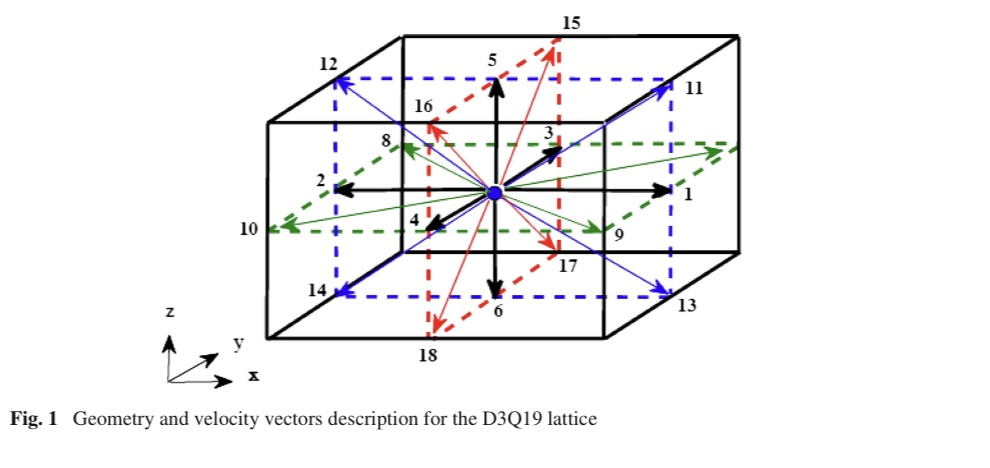
\includegraphics[width=01\linewidth]{IMG_7156.jpeg}

    \label{fig:placeholder}
\end{figure}



Notons que toutes les quantités et les paramètres physiques sont désormais exprimés en unités de Boltzmann sur réseau, avec 
\(\Delta x = 1\, lu\) (unité de réseau) et un pas de temps de simulation 
\(\Delta t = 1\, ts\) (pas de temps).

Dans ce modèle, l’équation de Boltzmann discrétisée est formulée sous la forme de l’équation de propagation-collision :

\[
f_k(\mathbf{x}+e_k\Delta t,\, t+\Delta t)
=
f_k(\mathbf{x},t)
-
\frac{\Delta t}{\tau}
\left[
f_k(\mathbf{x},t)-f_k^{(eq)}(\mathbf{x},t)
\right]
\]

où $\tau$ représente le temps de relaxation et
$f_k^{(eq)}$ la fonction de distribution d’équilibre
associée au vecteur vitesse $e_k$ :

\begin{equation}
f_k^{(\text{eq})} = \omega_k \rho \left[ 1 + \frac{3(\mathbf{e}_k \cdot \mathbf{u})}{c^2} + \frac{9(\mathbf{e}_k \cdot \mathbf{u})^2}{2c^4} \right]
\label{eq:equilibrium}
\end{equation}
où \( \omega_k \) est un facteur de pondération défini par :
\begin{equation}
\omega_k =
\begin{cases} 
1/3 & k = 0 \\
1/18 & k = 1, \dots, 6 \\
1/36 & k = 7, \dots, 18
\end{cases}
\label{eq:omega}
\end{equation}
L’équation (8) est généralement mise en œuvre à travers deux étapes de calcul successives :

\begin{enumerate}
    \item Étape de collision :
\end{enumerate} 


L’étape de collision dans LBM modélise l’interaction locale entre particules. Elle fait tendre chaque fonction de distribution $f_k$vers sa valeur d’équilibre $f_k^{(eq)}$, selon un temps de relaxation $\tau$. Ce processus conserve localement la masse et la quantité de mouvement.

Équation de collision (modèle BGK) :


\[
f_k^{'}(\mathbf{x}, t) = f_k(\mathbf{x}, t) - \frac{1}{\tau} \left[ f_k(\mathbf{x}, t) - f_k^{(\text{eq})}(\mathbf{x}, t) \right]
\]

\textbf{Équation d'équilibre (développement de Maxwell-Boltzmann discrétisé) :}

\[
f_k^{(\text{eq})} = \rho \, w_k \left[ 1 + \frac{\mathbf{c}_k \cdot \mathbf{u}}{c_s^2} + \frac{(\mathbf{c}_k \cdot \mathbf{u})^2}{2c_s^4} - \frac{\mathbf{u}^2}{2c_s^2} \right]
\]

\textbf{Moments locaux :}

\[
\rho = \sum_k f_k, \quad \rho \mathbf{u} = \sum_k f_k\mathbf{c}_k
\]



La collision est suivie de l'étape de propagation (streaming) 


\begin{enumerate}
    \item Étape de propagation :
\end{enumerate}
\begin{equation}
f_k(\mathbf{x} + \mathbf{e}_k \Delta t, t + \Delta t) = f'_k(\mathbf{x}, t)
\label{eq:streaming}
\end{equation}
La densité \( \rho \) et la vitesse d’écoulement \( \mathbf{u} \) sont calculées par :
\begin{equation}
\rho \mathbf{u} = \sum_k f_k \mathbf{e}_k
\label{eq:momentum}
\end{equation}

\begin{equation}
\rho = \sum_k f_k
\label{eq:density}
\end{equation}
et la pression \( p \) est exprimée par l’équation d’état des gaz parfaits :
\begin{equation}
p = c_s^2 \rho
\label{eq:pressure}
\end{equation}



où \( c_s \) est la vitesse du son et est liée à la vitesse du réseau \( c \) par :
\begin{equation}
c_s = c / \sqrt{3}
\end{equation}

La viscosité cinématique est reliée au temps de relaxation unique \( \tau \) par :

\begin{equation}
\nu = c_s^2 \left( \tau - \frac{1}{2} \right)
\end{equation}

Les différentes sortes de conditions aux limites peuvent être utilisées. 
Les conditions de Dirichlet et de Neumann sont imposées en utilisant la formulation proposée par Zou et He (1997). 
Pour la condition de non-glissement, deux schémas sont utilisés : un schéma classique de rebond complet dit \textit{full-way bounce-back} noté LBM--FBB, 
et un schéma de rebond interpolé linéaire noté LBM--IBB.

La technique du rebond (\textit{bounce-back}) peut être vue comme une équation de collision modifiée qui réfléchit les fonctions de distribution \( f_k \) dans la direction opposée \( \bar{e}_k \) telle que \( \bar{e}_k = -e_k \). 
Dans le modèle full-way bounce-back, la frontière est située approximativement à mi-distance entre le nœud solide et le nœud fluide voisin, mais sa position exacte dépend de la viscosité (Pan et al., 2006).

Le schéma de rebond interpolé étend la méthode du demi-pas (\textit{halfway bounce-back}) afin de prendre en compte la position exacte de la frontière physique. 
Si l’on note \( x_f \) le nœud fluide au voisinage de la frontière, tel que \( x_s = x_f + \Delta x \) soit un nœud solide, et \( x + dx \) un point situé sur la frontière solide (Fig. 2a), le schéma de rebond interpolé linéaire peut s’exprimer comme suit (Pan et al., 2006) :

Pour \( dx < \Delta x / 2 \),
\begin{equation}
f_k \left( \mathbf{x}_f, t + \Delta t \right) = 2 \frac{d_x}{\Delta x} f'_k \left( \mathbf{x}_f, t \right) + \left( 1 - 2 \frac{d_x}{\Delta x} \right) f'_k \left( \mathbf{x}_f - \Delta x, t \right)
\label{eq:interp1}
\end{equation}

and for \( d_x \geq \Delta x / 2 \),

\begin{equation}
f_k \left( \mathbf{x}_f, t + \Delta t \right) = \frac{\Delta x}{2d_x} f'_k \left( \mathbf{x}_f, t \right) + \frac{2d_x - \Delta x}{2d_x} f'_k \left( \mathbf{x}_f, t \right)
\label{eq:interp2}
\end{equation}

Le schéma BGK (Bhatnagar--Gross--Krook) est un modèle de collision utilisé dans la méthode de Boltzmann sur réseau.

L’équation BGK s’écrit :

\[
f_i(\mathbf{x}+\mathbf{e}_i \Delta t,t+\Delta t)-f_i(\mathbf{x},t)
=
-\frac{1}{\tau}
\left(
f_i(\mathbf{x},t)-f_i^{eq}(\mathbf{x},t)
\right)
\]

où :

\begin{itemize}
    \item $f_i$ : fonction de distribution,
    \item $f_i^{eq}$ : fonction de distribution à l’équilibre,
    \item $\tau$ : temps de relaxation,
    \item $\mathbf{e}_i$ : vecteur de vitesse discrète.
\end{itemize}

Le modèle BGK suppose que le système évolue progressivement vers un état d’équilibre après les collisions.
\section{Méthodes de traitement des frontières}
Les méthodes de frontière immergée sont classiquement divisées en deux catégories : les approches à interface nette (sharp interface) et les approches à interface diffuse (diffuse interface). Une méthode typique à interface nette est la méthode de forçage direct, qui consiste à maintenir une frontière étroite par l’utilisation de forces singulières appliquées directement à l’interface. Les vitesses sont ajustées par interpolation afin de restituer exactement la vitesse imposée sur l’interface. Toutefois, lorsque la diffusion numérique est évitée, des oscillations parasites peuvent apparaître. Le forçage est introduit après la discrétisation et dépend donc fortement des schémas numériques utilisés.

Un autre exemple de méthode de frontière immergée à interface nette est l’approche cut-cell (Ye et al. 1999 ; Udaykumar et al. 2001), dans laquelle les cellules proches de la frontière immergée sont localement redéfinies afin de reconstruire rigoureusement les flux interfaciaux.

Concernant les méthodes à interface diffuse, une force fictive est introduite par des termes de forçage ou de pénalisation dans le voisinage de l’interface afin de représenter les effets des corps immergés. Le forçage est défini avant la discrétisation des équations, mais l’interface est étalée sur une certaine longueur de diffusion, ce qui introduit un biais numérique sur les nœuds voisins.

La méthode IBM à forçage continu, également appelée méthode IBM classique dans la revue de Fotis Sotiropoulos et Xiaolei Yang (2014), ainsi que la méthode de pénalisation, constituent quelques exemples d’approches diffuses.

Dans ce travail, une méthode de forçage direct sera retenue afin de conserver une interface fluide–solide nette et de maintenir un contrôle direct sur la précision numérique ainsi que sur les propriétés de conservation de la masse.

Comme indiqué dans l’introduction, le couplage avec la méthode IBM est réalisé par l’ajout d’une densité de force de frontière dans l’équation de quantité de mouvement. Par conséquent, l’équation (2) est modifiée comme suit :
\begin{equation}
\frac{\partial \mathbf{u}}{\partial t} + \mathbf{u}\cdot\nabla \mathbf{u}
=
-\frac{\nabla p}{\rho}
+
\nu \nabla^2 \mathbf{u}
+
\frac{\mathbf{g}}{\rho}
\end{equation}
où g représente le terme de forçage utilisé pour satisfaire la condition de non-glissement sur les frontières immergées. Ainsi, l’équation de Boltzmann discrète modifiée s’écrit comme suit :
\begin{equation}
f_k(\mathbf{x}+\mathbf{e}_k\Delta t,\, t+\Delta t)
=
f_k(\mathbf{x},t)
-
\frac{\Delta t}{\tau}
\left[
f_k(\mathbf{x},t)-f_k^{(\mathrm{eq})}(\mathbf{x},t)
\right]
+
g_k(\mathbf{x},t)\Delta t
\end{equation}
avec \( g_k(\mathbf{x}, t) \) le terme de forçage discret.

Fondamentalement, ce terme de forçage peut être considéré comme la force requise pour modifier 
la vitesse non perturbée \( \mathbf{u}^* \) au voisinage de l'interface. Cette correction 
est dérivée de la vitesse désirée \( \overline{\mathbf{U}} \) au nœud de la grille d'intérêt. 
Les nœuds de la grille où le forçage se produit sont ici les nœuds externes aux corps 
immergés (c'est-à-dire, les grains solides) à l'intérieur du domaine fluide, comme illustré 
à la Fig.~\ref{fig:2}.

La vitesse \( \overline{\mathbf{U}} \) est obtenue par interpolation entre la vitesse à la 
frontière physique \( \mathbf{U} \) (par exemple, une vitesse nulle pour une condition 
d'adhérence) et la vitesse dans le fluide en vrac \( \mathbf{u}_B^* \). Nous obtenons ainsi 
pour chaque composante \( \overline{U}_j \):

\begin{equation}
\overline{U}_j = \frac{U_j + d_j u_{B,j}^*}{1 + d_j}, \quad j = x, y, z
\label{eq:interpolation_vitesse}
\end{equation}
où \( \mathbf{d} \) représente le vecteur de distance entre l’interface physique et le nœud du réseau considéré, comme illustré à la Fig.~2 pour la direction \( x \). En raison de l’hypothèse sur les corps immergés.
\begin{figure}[H]
    \centering
    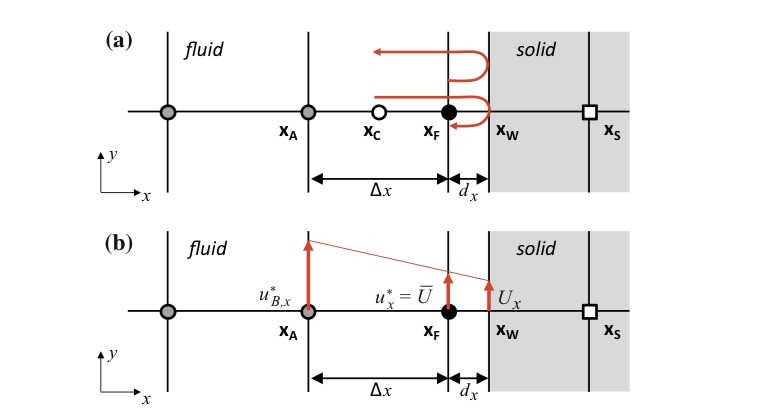
\includegraphics[width=0.5\linewidth]{IMG_7159.jpeg}
    \caption{Fig. 2 Illustration de la procédure d’interpolation dans la direction x, avec :a) la condition de rebond interpolé(Interpolated Bounce-Back, IBB) (schéma modifié d’après Peng et Luo, 2008) ,b) la méthode des frontières immergées (Immersed Boundary Method, IBM).}
    \label{fig:placeholder}
\end{figure}
\FloatBarrier
\begin{equation}
g_{k1}(\mathbf{x}, t^+) = \frac{\omega_k}{c_s^2} \mathbf{e}_k \cdot \mathbf{g}_1(\mathbf{x}, t^+)
\label{eq:gk1}
\end{equation}

\begin{equation}
\mathbf{g}_1(\mathbf{x}, t^+) = \rho(\mathbf{x}, t) \frac{\overline{\mathbf{U}}(\mathbf{x}, t^+) - \mathbf{u}^*(\mathbf{x}, t^+)}{\Delta t}
\label{eq:g1}
\end{equation}

Il convient de souligner que l'étape de forçage est introduite juste après la collision, comme décrit dans la procédure de calcul ci-dessous :

\textbf{Procédure de calcul de IB-LBM1 :}

1. Initialisation :
\begin{equation}
\rho(\mathbf{x}, t)\mathbf{u}(\mathbf{x}, t) = \sum_k f_k(\mathbf{x}, t)\mathbf{e}_k
\label{eq:init1}
\end{equation}

2. Étape de collision :
\begin{equation}
f_k'(\mathbf{x}, t^+) = f_k(\mathbf{x}, t) - \frac{1}{\tau} \left[ f_k(\mathbf{x}, t) - f_k^{(\text{eq})}(\mathbf{x}, t) \right]
\label{eq:collision1}
\end{equation}

\begin{equation}
\rho(\mathbf{x}, t)\mathbf{u}^*(\mathbf{x}, t^+) = \sum_k f_k'(\mathbf{x}, t^+)\mathbf{e}_k
\label{eq:ustar1}
\end{equation}

3. Étape de forçage :
\begin{equation}
f_k''(\mathbf{x}, t^+) = f_k'(\mathbf{x}, t^+) + \Delta t \, g_{k1}(\mathbf{x}, t^+)
\label{eq:forcing1}
\end{equation}

4. Étape de propagation (streaming) :
\begin{equation}
f_k(\mathbf{x} + \mathbf{e}_k \Delta t, t + \Delta t) = f_k''(\mathbf{x}, t^+)
\label{eq:streaming1}
\end{equation}

À l'inverse, pour la seconde méthode proposée par Kang and Hassan (2011) et appelée IB-LBM2, le terme de forçage est divisé pour être appliqué avant et après l'étape de collision. Les différentes étapes de calcul de la méthode sont résumées ci-dessous.

\textbf{Procédure de calcul de IB-LBM2 :}

1. Initialisation :
\begin{equation}
\rho(\mathbf{x}, t)\mathbf{u}^*(\mathbf{x}, t) = \sum_k f_k(\mathbf{x}, t)\mathbf{e}_k
\label{eq:init2}
\end{equation}

2. Première étape de forçage :
\begin{equation}
\rho(\mathbf{x}, t)\mathbf{u}(\mathbf{x}, t^-) = \sum_k f_k(\mathbf{x}, t)\mathbf{e}_k + \frac{\Delta t}{2} \mathbf{g}_2(\mathbf{x}, t)
\label{eq:forcing2}
\end{equation}

3. Étape de collision :
\begin{equation}
f_k'(\mathbf{x}, t^+) = f_k(\mathbf{x}, t) - \frac{1}{\tau} \left[ f_k(\mathbf{x}, t) - f_k^{(\text{eq})}(\mathbf{x}, t^-) \right]
\label{eq:collision2}
\end{equation}
4. Deuxième étape de forçage :
\begin{equation}
f_k''(\mathbf{x}, t^+) = f_k'(\mathbf{x}, t^+) + \Delta t \, g_{k2}(\mathbf{x}, t)
\label{eq:forcing2_2}
\end{equation}

5. Étape de propagation (streaming) :
\begin{equation}
f_k(\mathbf{x} + \mathbf{e}_k \Delta t, t + \Delta t) = f_k''(\mathbf{x}, t^+)
\label{eq:streaming2}
\end{equation}

et le terme de forçage s'exprime comme suit :

\begin{equation}
g_{k2}(\mathbf{x}, t) = \left(1 - \frac{1}{2\tau}\right) \omega_k \left[ 3 \frac{\mathbf{e}_k - \mathbf{u}(\mathbf{x}, t)}{c^2} + 9 \frac{\mathbf{e}_k \cdot \mathbf{u}(\mathbf{x}, t)}{c^4} \mathbf{e}_k \right] \cdot \mathbf{g}_2(\mathbf{x}, t)
\label{eq:gk2}
\end{equation}

où

\begin{equation}
\mathbf{g}_2(\mathbf{x}, t) = 2\rho(\mathbf{x}, t) \frac{\overline{\mathbf{U}}(\mathbf{x}, t) - \mathbf{u}^*(\mathbf{x}, t)}{\Delta t}
\label{eq:g2}
\end{equation}

Notons que la densité de force à la frontière \( g_{k2} \) peut être interprétée ici comme une correction des fonctions de distribution d'équilibre \( f_k^{(\text{eq})} \) de sorte que l'Éq. (20) vérifie rigoureusement l'équation LBKG classique, Éq. (8) (Guo et al. 2002).



\subsection{Exemple de Méthode des frontières immergées et méthode de Boltzmann sur réseau}

La méthode des frontières immergées (IBM) repose sur l’hypothèse suivante des frontières immergées proposée par Peskin~\cite{Peskin} : soit le domaine fluide--solide total
\[
\Omega \subset \mathbb{R}^{n}, \qquad (n=2,3)
\]
où $\Omega^{+}$ représente le domaine fluide et $\Omega^{-}$ représente le domaine solide.

Soit
\[
\Gamma = \Omega^{+} \cap \Omega^{-}
\]
l’interface immergée de couplage fluide--solide satisfaisant la condition de non-glissement, alors :
\[
\Omega = \Omega^{+} \cup \Omega^{-}.
\]

De plus, l’opérateur de diffusion (\textit{spread operator}) et l’opérateur d’interpolation (\textit{interpolation operator}) sont utilisés afin d’échanger les quantités physiques à l’interface, lesquels sont donnés par~\cite{ref33} :

\begin{equation}
f(\mathbf{x})=
\int_{\Gamma}
F(s)\,\delta(\mathbf{x}-\mathbf{X})\,ds
\label{eq1}
\end{equation}

\begin{equation}
U(\mathbf{X})=
\int_{\Omega}
u(\mathbf{x})\,\delta(\mathbf{x}-\mathbf{X})\,dx
\label{eq2}
\end{equation}

où
\[
\mathbf{x}=(x_i,\; i=1,2,3)\in\Omega
\]
désigne les coordonnées eulériennes, et
\[
s=(s_i,\; i=1,2,3)\in\Gamma
\]
désigne les coordonnées lagrangiennes des particules de l’interface.

L’application
\[
\mathbf{X}(s,t)\in\Omega
\]
correspond à la position eulérienne des particules caractérisées par les paramètres d’abscisse curviligne $s$ à l’instant $t$ ; $\delta(x)$ est la fonction delta ; $f$ et $u$ représentent respectivement la force et la vitesse sur les maillages eulériens du fluide ; tandis que $F$ et $U$ représentent la force et la vitesse sur les maillages lagrangiens du solide.

Pour le cas bidimensionnel, la fonction $\delta(x)$ est donnée par :

\begin{equation}
\delta(\mathbf{x})=\delta(x)\,\delta(y)
\label{eq3}
\end{equation}

Pour l’interpolation à cinq points~\cite{ref33}, $\delta(x)$ est définie par :

\begin{equation}
\delta(x)=
\begin{cases}
\dfrac{1}{8}
\left(
3-2|x|+\sqrt{1+4|x|-4x^{2}}
\right)
\\[0.3cm]
\dfrac{1}{8}
\left(
5-2|x|-\sqrt{-7+12|x|-4x^{2}}
\right)
\\[0.3cm]
0
\end{cases}
\label{eq4}
\end{equation}

La fonction lissée de $\delta(x)$ est donnée par :

\begin{equation}
\delta^{r}(x)=
\begin{cases}
\dfrac{1}{4}
\left(
1+\cos\left(\dfrac{\pi x}{2}\right)
\right),
& |x|\leq 2
\\[0.3cm]
0,
& |x|>2
\end{cases}
\label{eq5}
\end{equation}

Selon la théorie cinétique des gaz, l’équation continue de Boltzmann décrit le domaine fluide. L’équation de Boltzmann--BGK s’écrit~\cite{ref34} :

\begin{equation}
\frac{\partial f}{\partial t}
+
\boldsymbol{\xi}\cdot\nabla_{x}f
+
\mathbf{a}\cdot\nabla_{\xi}f
=
-\frac{1}{\tau_c}
\left[
f-f^{(eq)}
\right]
\label{eq6}
\end{equation}

où
\[
f=f(x,\xi,t)
\]
est la fonction de distribution des particules, $x$ est le vecteur position spatiale, $\xi$ est le vecteur vitesse, $t$ est le temps, $f^{(eq)}$ est la fonction de distribution à l’équilibre, $\tau_c$ est le temps de relaxation, et
\[
-\frac{1}{\tau_c}
\left[
f-f^{(eq)}
\right]
\]
est l’opérateur de collision BGK.

L’équation de Boltzmann sur réseau constitue une forme discrète de l’équation continue de Boltzmann obtenue à l’aide d’un schéma de discrétisation particulier~\cite{ref35}.
\section{Modèle couplé écoulement–transport}
À présent, nous considérons le couplage entre l’écoulement du fluide et le transport réactif dans un milieu poreux évoluant au cours du temps. Une grande diversité de situations réactives peut être rencontrée dans les applications souterraines : réaction hétérogène à l’interface fluide–solide, réaction homogène entre deux (ou plusieurs) espèces chimiques à l’intérieur d’une phase ou d’une région du milieu poreux, etc.

Sans perte de généralité, nous concentrons notre étude sur un système à deux régions dans lequel une seule espèce chimique est transportée par advection et diffusion dans le domaine fluide $\Omega_f(t)$ , et diffuse dans une région perméable $\Omega_r(t)$  (par exemple, des grains solides recouverts d’une fine couche de biofilm) où la réaction a lieu.

L’interface $\Sigma(t) $ entre les deux régions est supposée évoluer au cours du temps, mais suffisamment lentement pour qu’une approximation en régime quasi-stationnaire puisse être adoptée.

Sous ces hypothèses, les équations de bilan de masse pour le système à deux régions, combinées aux équations (2)–(5), prennent la forme suivante :
\begin{align}
\nabla \cdot (\mathbf{u}c_f) &= \nabla \cdot (D_f \nabla c_f), && \text{dans } \Omega_f \tag{36}\\
0 &= \nabla \cdot (D_r \nabla c_r) - R_c, && \text{dans } \Omega_r \tag{37}\\
D_f \nabla c_f \cdot \mathbf{n} &= D_r \nabla c_r \cdot \mathbf{n}, && \text{sur } \Sigma(t) \tag{38}\\
c_f &= c_r, && \text{sur } \Sigma(t) \tag{39}\\
c_f &= C_{\Gamma_1}, \quad c_r = C_{\Gamma_1}, && \text{sur } \Gamma_1 \tag{40}\\
D_f \nabla c_f \cdot \mathbf{n} &= \Phi_{\Gamma_2}, \quad D_f \nabla c_r \cdot \mathbf{n} = \Phi_{\Gamma_2}, && \text{sur } \Gamma_2 \tag{41}
\end{align}

où $c_f$ (resp. $c_r$) est la concentration du soluté dans $\Omega_f$ 
(resp. $\Omega_r$), $\mathbf{u}$ est le champ de vitesse prédit à partir 
des équations (2)--(5), et $D_f$ et $D_r$ sont les coefficients de diffusion 
dans $\Omega_f$ et $\Omega_r$. $R_c$ est le terme de réaction, décrit par 
une cinétique du premier ordre pour simplifier. Les conditions de Dirichlet 
et de Neumann sont imposées classiquement sur les frontières externes du domaine.

Comme précédemment pour le calcul de l'écoulement, des méthodes ne nécessitant 
pas un maillage conforme aux frontières sont requises pour simuler les champs 
de concentration à l'échelle du pore en raison de la croissance (ou diminution) 
de $\Omega_r$. Différentes techniques numériques ont été développées pour 
traiter de telles situations.
Les applications de dissolution/précipitation ont été étudiées dans plusieurs travaux, et l’on retrouve essentiellement les mêmes types de méthodes présentées précédemment pour le calcul de l’écoulement sur un maillage non conforme au corps : méthode ALE, approche VOF ou méthode de reconstruction d’interface. Comme précédemment, le choix de la méthode la plus adaptée dépend de plusieurs paramètres : complexité de la géométrie (domaine 2D ou 3D, instabilité de la forme de l’interface), réaction hétérogène ou homogène, étendue du front de réaction (front net ou diffus), par exemple.

Nous considérons ici deux méthodes différentes pour traiter ce problème numérique. Dans les deux cas, un schéma de discrétisation en volumes finis est utilisé.

Tout d’abord, un modèle de type volume de fluide est considéré. Il est basé sur l’approximation selon laquelle le comportement du système est proche de l’équilibre. Sous l’hypothèse que les temps caractéristiques de transport sont du même ordre de grandeur dans les deux régions et que le temps caractéristique de la cinétique de réaction est grand, la condition d’équilibre local de masse est valable. En d’autres termes, les gradients de concentration au voisinage de l’interface sont suffisamment faibles. Les concentrations ne varient pas significativement à l’échelle des cellules immergées. Par conséquent, une seule concentration $C$ peut être définie dans $\Omega_f$ et $\Omega_r$. Cette approximation conduit à un modèle de transport à une seule équation valable partout :

\begin{align}
\nabla \cdot (\mathbf{u}_{\phi} C) &= \nabla \cdot (D_{\phi} \nabla C) - R_{\phi},
&& \text{dans } \Omega = \Omega_f \cup \Omega_r \tag{42} \\
C &= C_{\Gamma_1}(\phi),
&& \text{sur } \Gamma_1 \tag{43} \\
D_{\phi}\nabla C \cdot \mathbf{n} &= \Phi_{\Gamma_2}(\phi),
&& \text{sur } \Gamma_2 \tag{44}
\end{align}

où $\phi(x,t)$ décrit la fraction volumique de $\Omega_r$ sur $\Omega$. 
$D_{\phi}$, $R_{\phi}$ et $\mathbf{u}_{\phi}$ représentent respectivement le coefficient de diffusion, le terme de réaction et le vecteur vitesse dans $\Omega$. Ils sont exprimés en fonction de $\phi$ de sorte que, pour les deux cas limites $\phi=0$ et $\phi=1$, les équations (36) et (37) sont retrouvées. Un commentaire similaire s’applique aux conditions aux limites externes sur $\Gamma_1$ et $\Gamma_2$. Ainsi, on obtient :

\begin{align}
D_{\phi}(x,t) &= \phi(x,t)D_r + \bigl(1-\phi(x,t)\bigr)D_f,
\tag{45} \\
R_{\phi}(x,t) &= \phi(x,t)R_c(x,t),
\tag{46} \\
\mathbf{u}_{\phi}(x,t) &= \bigl(1-\phi(x,t)\bigr)\mathbf{u}(x,t).
\tag{47}
\end{align}

Le revers de l’extrême simplicité de ce modèle est son domaine de validité limité. En effet, pour des vitesses élevées ou des taux de réaction élevés, l’équilibre local de masse n’est plus respecté, ce qui entraîne une diminution de la précision du modèle.

Dans le cas de fortes conditions de non-équilibre ou lorsqu’une estimation fine des flux interfaciaux est requise, des méthodes plus sophistiquées sont nécessaires. À titre d’exemple illustratif, une approche par reconstruction d’interface en volumes finis est utilisée dans ce travail afin d’éviter les procédures fastidieuses de fusion de cellules classiquement observées dans les formulations à cellules coupées.

Cette méthode implicite conduit à reconstruire les flux interfaciaux pour les cellules traversées par la frontière immergée. Cette étape de reconstruction, qui peut être particulièrement délicate en 3D, est relativement simple dans notre cas grâce à l’hypothèse d’interfaces planes par morceaux. Une interpolation linéaire est utilisée ici pour recalculer correctement les flux.

Une description de la procédure mathématique dans un cas unidimensionnel simplifié est détaillée ci-dessous afin de faciliter les calculs.

Tout d’abord, une description sur domaine unique est utilisée pour remplacer les équations (36) et (37) :

\begin{equation}
\nabla \cdot (\mathbf{U}C)=\nabla \cdot (D\nabla C)-R
\tag{48}
\end{equation}
\begin{figure}[H]
    \centering
    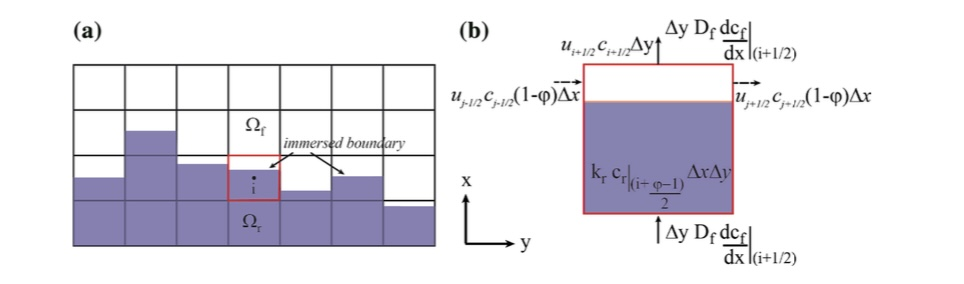
\includegraphics[width=1\linewidth]{IMG_7160.jpeg}
    
    \label{fig:placeholder}
\end{figure}
\FloatBarrier
La figure 3 montre : a) un maillage cartésien coupé par la frontière immergée ; 
b) le calcul des flux interfaciaux par la méthode de reconstruction de l’interface 
sur la cellule $i$.

où $U$, $D$ et $R$ sont des fonctions définies par morceaux. La discrétisation en volumes finis du flux diffusif, par exemple sur la cellule immergée unidimensionnelle représentée à la Fig.~3, conduit à l’intégration par morceaux suivante :

\begin{align}
\int_{i-\frac{1}{2}}^{i+\frac{1}{2}} 
\frac{\partial}{\partial x}
\left(
D \frac{\partial c}{\partial x}
\right) dx
&=
\int_{i-\frac{1}{2}+\phi}^{i+\frac{1}{2}}
\frac{\partial}{\partial x}
\left(
D_f \frac{\partial c_f}{\partial x}
\right) dx \nonumber \\
&\quad +
\int_{i-\frac{1}{2}}^{i-\frac{1}{2}+\phi}
\frac{\partial}{\partial x}
\left(
D_r \frac{\partial c_r}{\partial x}
\right) dx
\tag{49}
\end{align}

\begin{equation}
=
D_f \left.\frac{\partial c_f}{\partial x}\right|_{i+\frac{1}{2}}
-
D_r \left.\frac{\partial c_r}{\partial x}\right|_{i-\frac{1}{2}}
\tag{50}
\end{equation}

Ces flux interfaciaux doivent être interpolés correctement en tenant compte de la frontière immergée. Par exemple, pour $\phi(i)\geq 0.5$, on peut différencier le premier terme du membre de droite de l’équation (50) en utilisant le développement de Taylor :

\begin{equation}
c_f\Big|_{i+\frac{1}{2}}
=
c_f\Big|_{+}
+
\left.
\frac{\partial c_f}{\partial x}
\right|_{i+\frac{1}{2}}
(1-\phi(i))\Delta x
+
O(\delta x^2)
\tag{51}
\end{equation}

\begin{equation}
c_f\Big|_{i+\frac{1}{2}}
=
c_f\Big|_{i+1}
-
\left.
\frac{\partial c_f}{\partial x}
\right|_{i+\frac{1}{2}}
\frac{\Delta x}{2}
+
O(\delta x^2)
\tag{52}
\end{equation}

Les indices $+$ et $-$ désignent respectivement la position juste au-dessus et juste au-dessous de l’interface située en $i-\frac{1}{2}+\phi$.
Ici, $c_f|_+$ et $c_r|_-$ peuvent être calculés à partir des décompositions suivantes :

\begin{equation}
c_f\Big|_{+}
=
c_f\Big|_{i+1}
-
\left.
\frac{\partial c_f}{\partial x}
\right|_{+}
\left(
\frac{3}{2}-\phi(i)
\right)\Delta x
+
O(\delta x^2)
\tag{53}
\end{equation}

\begin{equation}
c_r\Big|_{-}
=
c_r\Big|_{i}
+
\left.
\frac{\partial c_r}{\partial x}
\right|_{-}
\left(
\phi(i)-\frac{1}{2}
\right)\Delta x
+
O(\delta x^2)
\tag{54}
\end{equation}

et à partir des conditions aux limites appropriées sur la frontière immergée :

\begin{equation}
D_f
\left.
\frac{\partial c_f}{\partial x}
\right|_{+}
=
D_r
\left.
\frac{\partial c_r}{\partial x}
\right|_{-}
\tag{55}
\end{equation}

\begin{equation}
c_f\Big|_{+}
=
c_r\Big|_{-}
\tag{56}
\end{equation}
Enfin, l'Éq. (50) peut être réécrite comme

\begin{equation}
\int_{i-\frac{1}{2}}^{i+\frac{1}{2}} \frac{\partial}{\partial x} D \left( \frac{\partial c}{\partial x} \right) dx = \frac{2 D_f D_r}{\Delta x} \left[ \frac{c_r|_{i+1} - c_r|_i}{D_r (3 - 2\phi(i)) + D_f (2\phi(i) - 1)} \right] 
- D_r \frac{c_r|_i - c_r|_{i-1}}{\Delta x}
\label{eq:57}
\end{equation}

De la même manière, le terme de réaction peut être exprimé comme

\begin{equation}
\int_{i-\frac{1}{2}}^{i+\frac{1}{2}} R \, dx = \int_{i-\frac{1}{2}}^{i-\frac{1}{2} + \phi} R_r \, dx
\label{eq:58}
\end{equation}

\begin{equation}
\approx k_r \, c_r|_{i + \frac{\phi - 1}{2}} \Delta x
\label{eq:59}
\end{equation}

où $k_r$ est la constante de vitesse cinétique du premier ordre et $c_r|_{i + \frac{\phi-1}{2}}$ est calculée par interpolation linéaire. Une reconstruction similaire s'applique pour le flux advectif, et l'extension en 3D est immédiate grâce à l'hypothèse sur la forme de l'interface.

Étant donné que l'utilisation des unités de Boltzmann sur réseau est parfois fastidieuse, nous définissons deux nombres adimensionnels, le nombre de Péclet et le nombre de Damköhler, que nous utiliserons dans la section suivante pour illustrer l'applicabilité de ces modèles :

\begin{equation}
Pe = \frac{V_m l_f}{D_f} \quad ; \quad Da = \frac{l_r^2 k_r}{D_r}.
\label{eq:60}
\end{equation}

où $V_m$ représente la vitesse moyenne dans la phase fluide et $l_f$ et $l_r$ sont les longueurs caractéristiques associées à $\Omega_f$ et $\Omega_r$.

% -------------------------
% CHAPITRE 4 — MÉTHODOLOGIE NUMÉRIQUE
% -------------------------

\chapter{Méthodologie numérique}
Ce chapitre présente la méthodologie numérique adoptée pour la simulation des écoulements réactifs dans des milieux poreux évolutifs, où la géométrie du domaine est susceptible de se modifier au cours du temps en raison des phénomènes de dissolution ou de précipitation. L’objectif principal est de décrire les outils numériques retenus pour modéliser de manière cohérente l’interaction entre l’écoulement du fluide, le transport des espèces chimiques dissoutes et l’évolution des interfaces solide–fluide.

La complexité de ces phénomènes réside dans le fort couplage entre plusieurs mécanismes physiques : d’une part, l’écoulement hydrodynamique est influencé par la géométrie instantanée du milieu poreux ; d’autre part, cette géométrie elle-même évolue sous l’effet des réactions chimiques à l’interface, modifiant progressivement les chemins d’écoulement ainsi que la distribution des concentrations. Une telle interaction nécessite une approche numérique capable de traiter simultanément les effets de transport, de réaction et de déplacement des frontières solides.

Dans ce contexte, la méthode de Boltzmann sur réseau (Lattice Boltzmann Method, LBM) constitue un cadre particulièrement adapté pour la simulation de l’écoulement dans des géométries complexes. Basée sur une description mésoscopique du fluide, elle permet de résoudre efficacement les équations de Navier–Stokes tout en conservant une grande souplesse dans le traitement des frontières irrégulières ou mobiles. Son architecture algorithmique, fondée sur les étapes successives de collision et de propagation, facilite également le couplage avec d’autres modèles physiques.

Le déplacement des interfaces solide–fluide est traité à l’aide de la méthode des frontières immergées (Immersed Boundary Method, IBM), qui permet de représenter des frontières mobiles sans reconstruire le maillage du domaine à chaque pas de temps. Deux variantes sont étudiées dans ce travail, notées IB–LBM1 et IB–LBM2. Elles reposent sur l’introduction de termes de forçage local destinés à imposer les conditions cinématiques sur la frontière mobile et à corriger localement le champ de vitesse. L’analyse comparative de ces deux formulations permet d’évaluer leur précision et leur robustesse dans le contexte de géométries évolutives.

Le transport réactif est modélisé par une approche spécifique permettant de suivre l’évolution des espèces dissoutes ainsi que les transformations de la phase solide. Deux méthodes sont mises en œuvre : la méthode Volume of Fluid (VOF), utilisée pour représenter la fraction volumique des phases, et la méthode de reconstruction (REC), employée pour redéfinir l’interface au cours de son évolution. Ces techniques assurent une représentation fidèle des changements topologiques du milieu tout en conservant la stabilité numérique du calcul.

Enfin, l’analyse du système repose sur l’introduction de nombres adimensionnels permettant de caractériser les régimes physiques dominants. Le nombre de Péclet compare les effets convectifs aux phénomènes diffusifs, tandis que le nombre de Damköhler mesure l’importance relative des réactions chimiques par rapport au transport. Ces paramètres jouent un rôle fondamental dans l’interprétation des mécanismes de dissolution et dans la comparaison des différents scénarios simulés.

Ce chapitre est organisé en quatre parties. La première décrit le schéma de résolution utilisé pour le calcul de l’écoulement. La deuxième présente le traitement des parois mobiles par la méthode des frontières immergées. La troisième détaille les méthodes de transport réactif mises en œuvre. Enfin, la dernière introduit les paramètres adimensionnels utilisés pour l’analyse physique des résultats.

\section{Schémas de résolution}
Schéma collision–streaming, calcul des vitesses, relaxation, viscosité.

La résolution numérique de l’écoulement est réalisée à l’aide de la méthode de Boltzmann sur réseau (LBM), fondée sur une approche mésoscopique de la dynamique des fluides. Cette méthode repose sur l’évolution temporelle des fonctions de distribution des particules sur un réseau discret, permettant de reconstruire les grandeurs macroscopiques telles que la densité et la vitesse.

Le principe général de la LBM consiste à décomposer chaque pas de temps en deux opérations successives : l’étape de collision et l’étape de propagation (\textit{streaming}). Cette structure algorithmique simple constitue l’un des principaux avantages de la méthode, en particulier pour le traitement des domaines complexes.

\subsection{Schéma collision--streaming}

L’équation de Boltzmann discrétisée avec opérateur BGK s’écrit :

\begin{equation}
f_i(\mathbf{x}+\mathbf{c}_i \Delta t,t+\Delta t)-f_i(\mathbf{x},t)
=
-\frac{1}{\tau}
\left[
f_i(\mathbf{x},t)-f_i^{eq}(\mathbf{x},t)
\right]
\end{equation}

où $f_i$ représente la fonction de distribution associée à la direction discrète $i$, $\mathbf{c}_i$ le vecteur vitesse discret, $\tau$ le temps de relaxation et $f_i^{eq}$ la fonction de distribution à l’équilibre.

La résolution s’effectue en deux étapes :

\paragraph{Étape de collision}

Les fonctions de distribution sont relaxées vers l’état d’équilibre :

\begin{equation}
f_i^{*}(\mathbf{x},t)
=
f_i(\mathbf{x},t)
-\frac{1}{\tau}
\left(
f_i(\mathbf{x},t)-f_i^{eq}(\mathbf{x},t)
\right)
\end{equation}

\paragraph{Étape de propagation}

Les distributions post-collision sont transportées vers les nœuds voisins :

\begin{equation}
f_i(\mathbf{x}+\mathbf{c}_i\Delta t,t+\Delta t)
=
f_i^{*}(\mathbf{x},t)
\end{equation}

\subsection{Calcul des grandeurs macroscopiques}

Les variables macroscopiques sont obtenues par sommation des fonctions de distribution :

\paragraph{Densité}

\begin{equation}
\rho
=
\sum_i f_i
\end{equation}

\paragraph{Vitesse}

\begin{equation}
\rho \mathbf{u}
=
\sum_i f_i \mathbf{c}_i
\end{equation}

où $\rho$ désigne la masse volumique et $\mathbf{u}$ le vecteur vitesse macroscopique.

\subsection{Distribution d’équilibre}

La fonction d’équilibre est donnée par :

\begin{equation}
f_i^{eq}
=
w_i \rho
\left[
1
+
\frac{\mathbf{c}_i \cdot \mathbf{u}}{c_s^2}
+
\frac{(\mathbf{c}_i \cdot \mathbf{u})^2}{2c_s^4}
-
\frac{\mathbf{u}^2}{2c_s^2}
\right]
\end{equation}

où $w_i$ sont les poids associés au réseau discret et $c_s$ la vitesse du son du réseau.

\subsection{Temps de relaxation et viscosité}

Le paramètre de relaxation $\tau$ contrôle la dissipation visqueuse du fluide. Il est relié à la viscosité cinématique par :

\begin{equation}
\nu
=
c_s^2
\left(
\tau-\frac{1}{2}
\right)\Delta t
\end{equation}

Dans le cas du réseau D2Q9, avec $\Delta x=\Delta t=1$, cette relation devient :

\begin{equation}
\nu
=
\frac{1}{3}
\left(
\tau-\frac{1}{2}
\right)
\end{equation}

Ainsi, le choix du temps de relaxation permet de fixer directement la viscosité du fluide simulé. La stabilité numérique impose généralement :

\begin{equation}
\tau > 0.5
\end{equation}

La méthode collision--streaming constitue ainsi le cœur du schéma de résolution hydrodynamique. Elle offre une formulation simple, locale et adaptée au couplage avec les méthodes de frontières immergées utilisées dans la suite de ce travail.

\section{Traitement des parois mobiles}

Dans le cadre de la simulation des milieux poreux évolutifs, la géométrie solide peut se déplacer ou se déformer au cours du temps sous l’effet des réactions chimiques à l’interface. Le traitement numérique de ces frontières mobiles représente une étape essentielle pour assurer un couplage correct entre l’écoulement et l’évolution du domaine.  

La méthode des frontières immergées (\textit{Immersed Boundary Method}, IBM) est utilisée pour représenter ces interfaces sans modifier la structure régulière du maillage eulérien. Les frontières solides sont décrites à l’aide de points lagrangiens immergés dans le réseau de calcul, et leur influence sur le fluide est introduite par un terme de forçage ajouté à l’équation de Boltzmann.  

Dans ce travail, deux formulations sont considérées : IB--LBM1 et IB--LBM2. Elles diffèrent essentiellement dans la manière de calculer la force d’interaction et la correction appliquée au champ de vitesse.

\subsection{Formulation du forçage}

Le forçage représente l’action de la frontière solide sur le fluide afin d’imposer localement la condition de non-glissement. Le terme de force volumique s’écrit :

\begin{equation}
\mathbf{F}(\mathbf{x},t)
=
\sum_{l}
\mathbf{F}_{l}(t)\,
\delta(\mathbf{x}-\mathbf{X}_{l})
\end{equation}

où $\mathbf{F}_{l}$ est la force appliquée au point lagrangien $l$, $\mathbf{X}_{l}$ sa position et $\delta$ la fonction delta discrète assurant l’interpolation entre la frontière et le réseau.

Dans l’approche de forçage direct, la force est calculée à partir de l’écart entre la vitesse imposée sur la frontière et la vitesse prédite du fluide :

\begin{equation}
\mathbf{F}_{l}
=
\frac{\mathbf{U}_{b}-\mathbf{u}^{*}}{\Delta t}
\end{equation}

où $\mathbf{U}_{b}$ est la vitesse imposée sur la frontière et $\mathbf{u}^{*}$ la vitesse intermédiaire obtenue avant correction.

\subsection{Méthode IB--LBM1}

La première approche applique directement la force calculée dans l’équation de Boltzmann. Le terme de forçage discret est ajouté sous la forme :

\begin{equation}
f_i(\mathbf{x}+\mathbf{c}_i\Delta t,t+\Delta t)
=
f_i^{*}(\mathbf{x},t)+g_i
\end{equation}

avec :

\begin{equation}
g_i
=
w_i
\left(
1-\frac{1}{2\tau}
\right)
\left[
\frac{\mathbf{c}_i-\mathbf{u}}{c_s^2}
+
\frac{(\mathbf{c}_i \cdot \mathbf{u})\mathbf{c}_i}{c_s^4}
\right]
\cdot
\mathbf{F}
\end{equation}

Cette formulation permet d’imposer la vitesse souhaitée en une seule correction explicite.

\subsection{Méthode IB--LBM2}

La seconde formulation introduit une correction itérative afin d’améliorer l’application de la condition de frontière, notamment lorsque la frontière est fortement courbée ou en mouvement rapide.

La vitesse corrigée est donnée par :

\begin{equation}
\mathbf{u}^{n+1}
=
\mathbf{u}^{*}
+
\frac{\Delta t}{\rho}\mathbf{F}
\end{equation}

Le calcul de la force est alors répété jusqu’à convergence de la vitesse imposée sur la frontière.

Cette approche permet une meilleure précision locale, au prix d’un coût de calcul plus élevé.

\subsection{Correction de vitesse}

Après application de la force, la vitesse macroscopique est recalculée :

\begin{equation}
\rho \mathbf{u}
=
\sum_i f_i \mathbf{c}_i
+
\frac{\Delta t}{2}\mathbf{F}
\end{equation}

Cette correction garantit la cohérence entre la distribution microscopique et la vitesse imposée au voisinage de la paroi mobile.

La vitesse aux points lagrangiens est obtenue par interpolation :

\begin{equation}
\mathbf{U}_{l}
=
\sum_{\mathbf{x}}
\mathbf{u}(\mathbf{x})
\delta(\mathbf{x}-\mathbf{X}_{l})
\Delta x^2
\end{equation}

Cette étape permet de vérifier la satisfaction de la condition cinématique sur la frontière.

\subsection{Procédure algorithmique}

La résolution complète d’un pas de temps avec la méthode IB s’effectue selon les étapes suivantes :

\begin{enumerate}
\item Calcul des distributions à l’équilibre.
\item Étape de collision.
\item Calcul de la vitesse intermédiaire.
\item Interpolation vers les points lagrangiens.
\item Évaluation de la force de correction.
\item Projection de la force sur le réseau eulérien.
\item Mise à jour des fonctions de distribution.
\item Propagation (\textit{streaming}).
\item Recalcul des grandeurs macroscopiques.
\item Mise à jour de la position de la frontière.
\end{enumerate}

L’algorithme est répété à chaque pas de temps, ce qui permet de suivre l’évolution de la frontière solide sans reconstruction du maillage.

La combinaison IB--LBM constitue ainsi un outil particulièrement adapté pour l’étude des écoulements couplés à l’évolution géométrique des structures poreuses.

\section{Méthodes de transport réactif}

Dans les systèmes poreux réactifs, l’écoulement du fluide, le transport des espèces dissoutes et les réactions chimiques à l’interface solide--fluide sont fortement couplés. La dissolution ou la précipitation modifie progressivement la géométrie du milieu, ce qui influence à son tour la dynamique de l’écoulement et la distribution des concentrations. La modélisation numérique de ce phénomène nécessite donc une méthode capable de suivre simultanément l’évolution des interfaces et les mécanismes de transport.

Dans ce travail, le suivi de l’évolution de la phase solide est assuré par la méthode \textit{Volume of Fluid} (VOF), tandis que la reconstruction géométrique de l’interface est réalisée par la méthode de reconstruction (REC). Ces deux approches permettent de représenter l’évolution continue des frontières solides dans un cadre eulérien.

\subsection{Principe du transport réactif}

Le transport d’une espèce dissoute dans le fluide est régi par l’équation générale de convection--diffusion--réaction :

\begin{equation}
\frac{\partial C}{\partial t}
+
\nabla \cdot (\mathbf{u}C)
=
\nabla \cdot (D \nabla C)
+
R(C)
\end{equation}

où $C$ désigne la concentration de l’espèce transportée, $\mathbf{u}$ la vitesse du fluide, $D$ le coefficient de diffusion moléculaire et $R(C)$ le terme de réaction chimique.

Le terme convectif représente le transport par advection, le terme diffusif traduit le mélange moléculaire et le terme source décrit les échanges liés aux réactions de surface.

Lorsque la réaction se produit uniquement à l’interface solide--fluide, la cinétique peut être exprimée sous la forme :

\begin{equation}
R_s
=
k_r(C-C_s)
\end{equation}

où $k_r$ est la constante cinétique et $C_s$ la concentration d’équilibre à la surface.

Cette relation détermine le flux de matière transféré entre la phase solide et la phase fluide.

\subsection{Méthode Volume of Fluid (VOF)}

La méthode VOF est utilisée pour suivre l’évolution volumique de la phase solide. Chaque cellule du domaine est associée à une variable scalaire $\phi$ représentant la fraction volumique solide :

\begin{equation}
\phi
=
\frac{V_s}{V_c}
\end{equation}

où $V_s$ est le volume solide contenu dans la cellule et $V_c$ le volume total de la cellule.

La variable $\phi$ vérifie :

\begin{equation}
0 \leq \phi \leq 1
\end{equation}

Les trois états possibles sont :

\begin{itemize}
\item $\phi = 1$ : cellule entièrement solide,
\item $\phi = 0$ : cellule entièrement fluide,
\item $0<\phi<1$ : cellule interfaciale.
\end{itemize}

Cette représentation permet de décrire la géométrie sans reconstruire le maillage.

\subsection{Évolution de la fraction volumique}

La variation de la fraction solide est liée à la réaction de dissolution :

\begin{equation}
\frac{\partial \phi}{\partial t}
=
-\frac{R_s A_s}{\rho_s V_c}
\end{equation}

où $A_s$ est l’aire interfaciale locale et $\rho_s$ la masse volumique du solide.

Sous forme discrète :

\begin{equation}
\phi^{n+1}
=
\phi^n
-
\frac{R_s A_s}{\rho_s V_c}\Delta t
\end{equation}

Cette relation traduit la réduction progressive du volume solide sous l’effet de la réaction.

Lorsqu’une cellule atteint :

\begin{equation}
\phi = 0
\end{equation}

elle devient totalement fluide et participe alors à l’écoulement.

\subsection{Flux réactif interfacial}

Le flux de dissolution à l’interface peut s’écrire :

\begin{equation}
J
=
-k_r(C_s-C_{eq})
\end{equation}

Le flux diffusif au voisinage de la paroi est :

\begin{equation}
J_d
=
-D
\frac{\partial C}{\partial n}
\end{equation}

La continuité impose :

\begin{equation}
-D
\frac{\partial C}{\partial n}
=
k_r(C_s-C_{eq})
\end{equation}

Cette relation constitue la condition limite réactive utilisée pour coupler le transport et l’évolution de la phase solide.

\subsection{Méthode de reconstruction (REC)}

La méthode REC est utilisée pour reconstruire localement l’interface après modification de la fraction volumique.

Le vecteur normal à l’interface est obtenu par :

\begin{equation}
\mathbf{n}
=
\frac{\nabla \phi}{|\nabla \phi|}
\end{equation}

avec :

\begin{equation}
\nabla \phi
=
\left(
\frac{\partial \phi}{\partial x},
\frac{\partial \phi}{\partial y}
\right)
\end{equation}

La position de l’interface est déterminée en conservant le volume solide correspondant à la nouvelle valeur de $\phi$.

Cette reconstruction assure :

\begin{itemize}
\item conservation du volume,
\item continuité géométrique,
\item représentation précise des fronts de dissolution.
\end{itemize}

\subsection{Déplacement de l’interface}

La vitesse normale de déplacement est définie par :

\begin{equation}
V_n
=
\frac{J}{\rho_s}
\end{equation}

soit :

\begin{equation}
V_n
=
\frac{k_r(C_s-C_{eq})}{\rho_s}
\end{equation}

Le déplacement pendant un pas de temps vaut :

\begin{equation}
\Delta s
=
V_n \Delta t
\end{equation}

La nouvelle position est :

\begin{equation}
\mathbf{X}^{n+1}
=
\mathbf{X}^{n}
+
V_n \mathbf{n}\Delta t
\end{equation}

Cette mise à jour est appliquée aux cellules interfaciales.

\subsection{Couplage avec l’écoulement}

Après modification de la géométrie, le champ d’écoulement est recalculé.

Le couplage s’effectue selon la séquence :

\begin{enumerate}
\item résolution de l’écoulement,
\item calcul du champ de concentration,
\item évaluation de la réaction,
\item mise à jour de $\phi$,
\item reconstruction de l’interface,
\item mise à jour de la géométrie,
\item recalcul de l’écoulement.
\end{enumerate}

Ce cycle est répété à chaque pas de temps.

\subsection{Conditions de validité}

La stabilité numérique impose plusieurs contraintes.

Le déplacement interfacial doit rester inférieur à la maille :

\begin{equation}
V_n\Delta t < \Delta x
\end{equation}

La diffusion doit être correctement résolue :

\begin{equation}
\frac{D\Delta t}{\Delta x^2}<1
\end{equation}

Le transport convectif doit satisfaire :

\begin{equation}
\frac{u\Delta t}{\Delta x}<1
\end{equation}

La résolution géométrique exige :

\begin{equation}
\Delta x \ll L_c
\end{equation}

où $L_c$ est l’échelle caractéristique de l’interface.

Enfin, la variation volumique doit rester faible :

\begin{equation}
|\phi^{n+1}-\phi^n| \ll 1
\end{equation}

afin d’éviter une perte de précision.

\subsection{Avantages de l’approche}

L’association VOF--REC présente plusieurs avantages :

\begin{itemize}
\item suivi continu des interfaces,
\item conservation de la masse solide,
\item compatibilité avec les géométries complexes,
\item couplage naturel avec LBM,
\item adaptation aux milieux poreux évolutifs.
\end{itemize}

Cette approche constitue ainsi une méthode robuste pour la simulation des phénomènes de dissolution dans les structures poreuses soumises au transport réactif.

\section{Paramètres adimensionnels}

Dans l’étude des phénomènes de transport réactif en milieu poreux, les paramètres adimensionnels jouent un rôle fondamental dans l’analyse des mécanismes physiques gouvernant l’évolution du système. Ils permettent de comparer des phénomènes de nature différente — convection, diffusion et réaction chimique — en éliminant l’influence directe des unités physiques. Cette approche facilite l’interprétation des résultats numériques, la comparaison entre différents cas d’étude et l’identification des régimes dominants.

Les processus simulés dans ce travail impliquent l’interaction entre l’écoulement du fluide, le transport des espèces dissoutes et la dissolution progressive de la matrice solide. Le comportement du système dépend principalement de la compétition entre les mécanismes de transport et la vitesse des réactions de surface. Deux nombres adimensionnels sont particulièrement importants : le nombre de Péclet et le nombre de Damköhler.

\subsection{Nombre de Péclet}

Le nombre de Péclet caractérise le rapport entre le transport convectif et le transport diffusif. Il représente la capacité de l’écoulement à transporter les espèces dissoutes relativement à leur dispersion moléculaire.

Il est défini par :

\begin{equation}
Pe
=
\frac{UL}{D}
\end{equation}

où :

\begin{itemize}
\item $U$ désigne la vitesse caractéristique du fluide ;
\item $L$ représente la longueur caractéristique du système ;
\item $D$ est le coefficient de diffusion moléculaire.
\end{itemize}

Le nombre de Péclet peut être interprété comme le rapport entre deux échelles de temps caractéristiques.

Le temps d’advection est :

\begin{equation}
t_{adv}
=
\frac{L}{U}
\end{equation}

Le temps de diffusion est :

\begin{equation}
t_{diff}
=
\frac{L^2}{D}
\end{equation}

D’où :

\begin{equation}
Pe
=
\frac{t_{diff}}{t_{adv}}
\end{equation}

Cette relation montre que le nombre de Péclet compare la rapidité du transport convectif à celle de la diffusion.

\subsubsection{Signification physique}

Lorsque :

\begin{equation}
Pe \ll 1
\end{equation}

la diffusion domine. Les espèces dissoutes se répartissent uniformément dans le domaine, ce qui conduit à des réactions réparties sur toute l’interface.

Lorsque :

\begin{equation}
Pe \gg 1
\end{equation}

l’advection devient dominante. Le transport est orienté selon l’écoulement principal, ce qui favorise la formation de gradients de concentration marqués.

Lorsque :

\begin{equation}
Pe \approx 1
\end{equation}

les deux mécanismes contribuent simultanément.

\subsubsection{Influence sur la dissolution}

Le nombre de Péclet influence directement la morphologie de dissolution :

\begin{itemize}
\item faible $Pe$ : dissolution uniforme ;
\item $Pe$ intermédiaire : dissolution localisée ;
\item grand $Pe$ : apparition de canaux préférentiels.
\end{itemize}

Dans les milieux poreux, l’augmentation de $Pe$ favorise souvent l’apparition de structures ramifiées dues à la focalisation du flux.

\subsection{Nombre de Damköhler}

Le nombre de Damköhler mesure l’importance de la réaction par rapport au transport.

Il est défini par :

\begin{equation}
Da
=
\frac{k_rL}{U}
\end{equation}

où :

\begin{itemize}
\item $k_r$ est la constante cinétique de réaction ;
\item $L$ la longueur caractéristique ;
\item $U$ la vitesse caractéristique.
\end{itemize}

Il compare le temps de transport au temps de réaction.

Le temps réactionnel est :

\begin{equation}
t_{react}
=
\frac{1}{k_r}
\end{equation}

Ainsi :

\begin{equation}
Da
=
\frac{t_{adv}}{t_{react}}
\end{equation}

\subsubsection{Interprétation}

Si :

\begin{equation}
Da \ll 1
\end{equation}

la réaction est lente. Le système est gouverné par la cinétique chimique.

Si :

\begin{equation}
Da \gg 1
\end{equation}

la réaction est rapide. Le transport devient limitant.

Si :

\begin{equation}
Da \approx 1
\end{equation}

transport et réaction interagissent de manière équilibrée.

\subsubsection{Conséquences physiques}

Le nombre de Damköhler détermine la localisation des réactions :

\begin{itemize}
\item faible $Da$ : réaction distribuée ;
\item grand $Da$ : réaction concentrée sur certaines zones ;
\item très grand $Da$ : forte instabilité morphologique.
\end{itemize}

Dans les simulations de dissolution, un grand $Da$ favorise la concentration de la dissolution aux entrées des pores.

\subsection{Damköhler diffusif}

Pour les situations où la diffusion contrôle le transfert vers la surface, on introduit :

\begin{equation}
Da_{II}
=
\frac{k_rL^2}{D}
\end{equation}

Ce paramètre compare directement la vitesse de réaction à la diffusion moléculaire.

Il est lié à $Pe$ et $Da$ par :

\begin{equation}
Da_{II}
=
Pe \times Da
\end{equation}

Cette relation montre que le comportement global résulte du couplage entre les trois mécanismes.

\subsection{Mise sous forme adimensionnelle}

L’équation de transport :

\begin{equation}
\frac{\partial C}{\partial t}
+
\mathbf{u}\cdot\nabla C
=
D\nabla^2C
+
R
\end{equation}

est rendue adimensionnelle par :

\begin{equation}
x^{*}
=
\frac{x}{L}
\end{equation}

\begin{equation}
t^{*}
=
\frac{Ut}{L}
\end{equation}

\begin{equation}
C^{*}
=
\frac{C}{C_0}
\end{equation}

On obtient :

\begin{equation}
\frac{\partial C^{*}}{\partial t^{*}}
+
\mathbf{u}^{*}\cdot\nabla C^{*}
=
\frac{1}{Pe}\nabla^2C^{*}
+
Da\,R^{*}
\end{equation}

Cette écriture montre que l’évolution du système dépend principalement des valeurs de $Pe$ et $Da$.

\subsection{Régimes physiques}

La combinaison des deux nombres permet de définir plusieurs régimes.

\subsubsection{Faible $Pe$ et faible $Da$}

Le transport est diffusif et la réaction lente. La dissolution est homogène.

\subsubsection{Faible $Pe$ et grand $Da$}

La diffusion limite l’accès au réactif. L’évolution reste régulière.

\subsubsection{Grand $Pe$ et faible $Da$}

L’écoulement transporte rapidement les espèces mais la réaction reste lente.

\subsubsection{Grand $Pe$ et grand $Da$}

Le transport est fortement advectif et la réaction rapide. Des canaux de dissolution apparaissent.

\subsection{Rôle dans les simulations}

Les nombres adimensionnels sont utilisés pour :

\begin{itemize}
\item définir les conditions initiales ;
\item comparer différents scénarios ;
\item interpréter l’évolution des structures poreuses ;
\item analyser les transitions morphologiques ;
\item étudier la stabilité du front de dissolution.
\end{itemize}

Ils permettent également de relier les simulations numériques à des systèmes physiques réels, quelle que soit leur échelle.

\subsection{Importance dans cette étude}

Dans ce travail, le nombre de Péclet contrôle la structure du transport de masse, tandis que le nombre de Damköhler gouverne la vitesse de dissolution. Leur interaction détermine l’évolution géométrique du milieu poreux ainsi que la formation éventuelle de voies préférentielles d’écoulement.

Ces deux paramètres constituent donc les grandeurs essentielles pour interpréter les résultats obtenus et caractériser les différents régimes de dissolution étudiés.
% -------------------------
% CHAPITRE 5 — RÉSULTATS NUMÉRIQUES
% -------------------------

\chapter{Résultats numériques}
Ce chapitre est consacré à la présentation et à l’analyse des résultats numériques obtenus à l’aide de la méthodologie développée au chapitre précédent. L’objectif principal est d’évaluer la capacité du modèle couplé à reproduire de manière fidèle les phénomènes d’écoulement et de transport réactif dans des milieux poreux évolutifs. Une attention particulière est portée à la précision des méthodes numériques utilisées ainsi qu’à leur robustesse lorsque la géométrie du pore varie sous l’effet des réactions de dissolution.

La première partie concerne l’étude du modèle hydrodynamique. Les résultats issus des méthodes basées sur la méthode de Boltzmann sur réseau sont comparés à des solutions analytiques de référence afin de vérifier la validité du schéma numérique. L’influence de la résolution spatiale ainsi que de la taille caractéristique du pore est examinée afin d’évaluer la sensibilité du modèle aux variations géométriques. Cette étape permet également de quantifier l’erreur introduite par les différentes approches de traitement des interfaces solides.

Une analyse détaillée de l’erreur relative est ensuite réalisée à partir des résultats présentés dans l’article de référence. Cette comparaison met en évidence les limites des schémas classiques lorsque le pore devient très étroit ou lorsque la frontière solide présente une forte courbure. Les performances des deux formulations IB–LBM sont alors comparées afin d’identifier l’approche la plus adaptée aux géométries évolutives.

La deuxième partie est consacrée au transport réactif. Les résultats obtenus avec les méthodes VOF, REC et FVM sont confrontés afin d’analyser leur capacité à reproduire correctement la distribution des espèces dissoutes dans le domaine poreux. L’étude porte en particulier sur l’évolution des profils de concentration et sur la représentation de l’interface mobile au cours de la dissolution.

L’influence du nombre de Damköhler est également étudiée, car ce paramètre contrôle directement la compétition entre transport et réaction chimique. Les simulations permettent de distinguer différents régimes : pour des valeurs faibles, la dissolution reste relativement homogène, tandis que des valeurs élevées conduisent à la formation de gradients très marqués. Ces conditions mettent en évidence les performances respectives des méthodes numériques et leur aptitude à traiter des fronts fortement localisés.

Enfin, une analyse du coût numérique est présentée afin de comparer les différentes méthodes du point de vue du temps de calcul et de la précision obtenue. Cette comparaison permet de discuter le compromis entre efficacité numérique et qualité des résultats, critère essentiel pour la simulation de systèmes poreux complexes sur des temps longs.

L’ensemble des résultats présentés dans ce chapitre permet ainsi de valider les outils numériques développés, d’évaluer leur domaine d’application et de mettre en évidence les avantages des approches retenues pour l’étude des écoulements réactifs en milieu poreux évolutif.
\section{Étude du modèle d’écoulement}
\section{Étude du modèle d’écoulement}

Cette section a pour objectif d’évaluer les performances du modèle hydrodynamique développé à l’aide de la méthode de Boltzmann sur réseau couplée aux méthodes de frontières immergées. L’étude porte sur la précision de la résolution de l’écoulement dans des géométries poreuses évolutives, en particulier lorsque la taille des pores varie au cours du temps sous l’effet de la dissolution.

La validation du modèle est réalisée à partir de comparaisons avec des solutions analytiques de référence. Cette démarche permet de quantifier l’écart entre les solutions numériques et les solutions théoriques et d’identifier les limites de chaque méthode lorsque la géométrie devient fortement contrainte.

L’analyse se concentre sur deux aspects principaux : l’influence de la taille du pore et l’effet de la résolution spatiale. Ces deux paramètres jouent un rôle déterminant dans la qualité de la représentation des interfaces et dans la précision du champ de vitesse.

Dans le cadre de cette étude, trois approches sont comparées :

\begin{itemize}
\item la méthode classique LBM avec traitement standard de frontière ;
\item la formulation IB--LBM1 ;
\item la formulation IB--LBM2.
\end{itemize}

L’objectif est de déterminer la méthode la plus adaptée aux écoulements confinés dans des structures poreuses évolutives.

\subsection{Cadre de validation}

La configuration étudiée correspond à un écoulement dans un canal poreux dont la géométrie varie en fonction du rayon des grains solides. Cette configuration permet de reproduire les situations rencontrées lors de la dissolution progressive des pores.

Les simulations sont réalisées en régime laminaire permanent. L’écoulement est supposé incompressible et isotherme. Les conditions aux limites imposent :

\begin{itemize}
\item une vitesse imposée à l’entrée ;
\item une pression de sortie ;
\item une condition de non-glissement sur les parois solides.
\end{itemize}

La validation repose sur la comparaison des profils de vitesse obtenus numériquement avec la solution analytique disponible pour un écoulement de Poiseuille modifié par la présence d’obstacles.

La précision est évaluée selon l’erreur relative :

\begin{equation}
E_r
=
\frac{\|u_{num}-u_{ref}\|}{\|u_{ref}\|}
\end{equation}

où $u_{num}$ représente la solution numérique et $u_{ref}$ la solution analytique.

\subsection{Influence de la taille du pore}

La taille du pore constitue un paramètre géométrique essentiel car elle contrôle la section disponible pour l’écoulement. Lorsque le pore se rétrécit, les gradients de vitesse deviennent plus importants et la précision numérique dépend fortement de la représentation de l’interface.

Le diamètre hydraulique est défini par :

\begin{equation}
d_h
=
\frac{4A}{P}
\end{equation}

où $A$ est la section fluide et $P$ le périmètre mouillé.

La diminution de $d_h$ entraîne :

\begin{itemize}
\item une augmentation de la vitesse locale ;
\item une concentration du cisaillement près des parois ;
\item une amplification des erreurs de discrétisation.
\end{itemize}

Les résultats montrent que les méthodes classiques deviennent moins précises lorsque :

\begin{equation}
d_h \rightarrow 0
\end{equation}

car l’interface solide occupe une proportion importante du maillage.

Les formulations IB présentent une meilleure robustesse grâce à l’interpolation des conditions limites.

\subsection{Influence de la finesse du maillage}

La précision du modèle dépend également du nombre de nœuds utilisés pour discrétiser le domaine.

Le pas spatial est :

\begin{equation}
\Delta x
=
\frac{L}{N}
\end{equation}

où $N$ est le nombre de cellules dans la direction étudiée.

Lorsque $N$ augmente :

\begin{itemize}
\item la représentation de la frontière s’améliore ;
\item la précision des gradients augmente ;
\item l’erreur relative diminue.
\end{itemize}

Cependant, le coût de calcul augmente également.

L’erreur théorique suit :

\begin{equation}
E_r
\propto
(\Delta x)^p
\end{equation}

où $p$ représente l’ordre de convergence.

Les résultats indiquent que :

\begin{itemize}
\item LBM standard : convergence limitée ;
\item IB--LBM1 : amélioration intermédiaire ;
\item IB--LBM2 : meilleure convergence.
\end{itemize}

\subsection{Analyse des champs de vitesse}

Le champ de vitesse présente une forte sensibilité à la position des frontières.

La vitesse moyenne est calculée par :

\begin{equation}
\bar{u}
=
\frac{1}{A}
\int_A u \, dA
\end{equation}

Le profil longitudinal permet d’évaluer :

\begin{itemize}
\item la conservation du débit ;
\item la continuité hydrodynamique ;
\item la précision près des interfaces.
\end{itemize}

Les simulations montrent que :

\begin{itemize}
\item la méthode classique surestime la vitesse près des parois ;
\item IB--LBM1 réduit cette erreur ;
\item IB--LBM2 reproduit fidèlement le profil théorique.
\end{itemize}

\subsection{Sensibilité à la géométrie évolutive}

Dans un milieu poreux évolutif, la géométrie change au cours du temps.

La position de l’interface est :

\begin{equation}
\Gamma(t)
\end{equation}

La variation de cette frontière modifie localement la distribution du flux.

Le débit volumique est :

\begin{equation}
Q
=
\int_A u\,dA
\end{equation}

Lorsque la dissolution élargit le pore :

\begin{equation}
Q(t)
\uparrow
\end{equation}

Les méthodes IB permettent de suivre cette évolution sans remeshing.

\subsection{Discussion des résultats}

Les comparaisons montrent clairement que la qualité du traitement des interfaces conditionne la précision globale.

Les principales observations sont :

\begin{itemize}
\item amélioration significative avec IB ;
\item réduction de l’erreur pour les pores étroits ;
\item meilleure stabilité avec IB--LBM2 ;
\item meilleure représentation des interfaces courbes.
\end{itemize}

La méthode IB--LBM2 apparaît particulièrement adaptée aux simulations de dissolution, car elle maintient la précision même lorsque les pores deviennent très fins.

Cette robustesse constitue un avantage essentiel pour les simulations couplées transport--réaction présentées dans la section suivante.
\subsection{Comparaison avec la solution analytique}
Influence de la taille du pore et de la finesse du maillage.

\subsection{Analyse de l’erreur relative}
Résultats basés sur les figures et tableaux de l’article:
\begin{itemize}
    \item Amélioration notable par IB–LBM2.
    \item Dégradation des méthodes classiques lorsque le pore se resserre.
\end{itemize}

\section{Étude du transport réactif}
\subsection{Comparaison VOF / REC / FVM}
Analyse des profils de concentration.

\subsection{Effet du nombre de Damköhler}
Da faible : profils lisses.  
Da élevé : forts gradients → REC plus précis.

\section{Analyse du coût numérique}
Discussion CPU vs précision.

% -------------------------
% CHAPITRE 6 — DISCUSSION
% -------------------------

\chapter{Discussion}
Dans cette section, nous évaluons l’efficacité des méthodes de frontières immergées pour le calcul simultané de l’écoulement et du transport de soluté dans une géométrie poreuse évoluant au cours du temps. À cette fin, nous considérons un pore unique tridimensionnel à section carrée. Ce type de géométrie est classiquement utilisé pour la validation de la méthode de Boltzmann sur réseau (LBM) (Maier et al. 1996 ; Zou et He 1997 ; Strack et Cook 2007).

Les parois de ce pore sont supposées évoluer avec le temps, de sorte que les frontières physiques ne coïncident pas avec le maillage numérique, comme illustré à la Fig.~4. La grandeur $l$ représente le col du pore, dont la largeur diminue au cours du temps. La quantité $2h$ correspond à la largeur totale du domaine, tandis que $H$ désigne l’épaisseur des parois mobiles, de telle sorte que :

\begin{equation}
2h = 2H + l
\end{equation}

Un maillage initial de $40 \times 40$ nœuds est considéré sur la section carrée de largeur $2h$.

Il convient de préciser que le couplage avec l’évolution de l’interface n’est pas pris en compte dans le présent travail. Afin de comparer les différents modèles dans des conditions similaires, on suppose implicitement un colmatage uniforme du pore avec une approximation en régime quasi-stationnaire. Ainsi, la comparaison des écoulements est effectuée pour une même géométrie à différentes tailles de col de pore, sans nécessiter la résolution d’une équation différentielle supplémentaire.

Nous limitons l’analyse à des conditions d’écoulement en régime quasi-stationnaire. Une condition de pression constante est imposée à l’entrée et à la sortie, avec :

\begin{equation}
\Delta p = 10^{-4} \cdot c_s^2
\end{equation}

Il convient de souligner que cette condition de pression constante entraîne une diminution de la vitesse moyenne du fluide lorsque le pore se rétrécit.

La viscosité cinématique est fixée à :

\begin{equation}
\nu = \frac{1}{6}
\end{equation}

Compte tenu du gradient de pression imposé à l’échelle du pore ainsi que de la plage de variation de la taille du col, le nombre de Reynolds résultant varie entre :

\begin{equation}
10^{-5} \le Re \le 2 \times 10^{-4}
\end{equation}

Ces très faibles valeurs du nombre de Reynolds correspondent à un écoulement de Stokes pur, ce qui constitue la situation typique des écoulements dans les milieux poreux.
\begin{figure}[H]
    \centering
    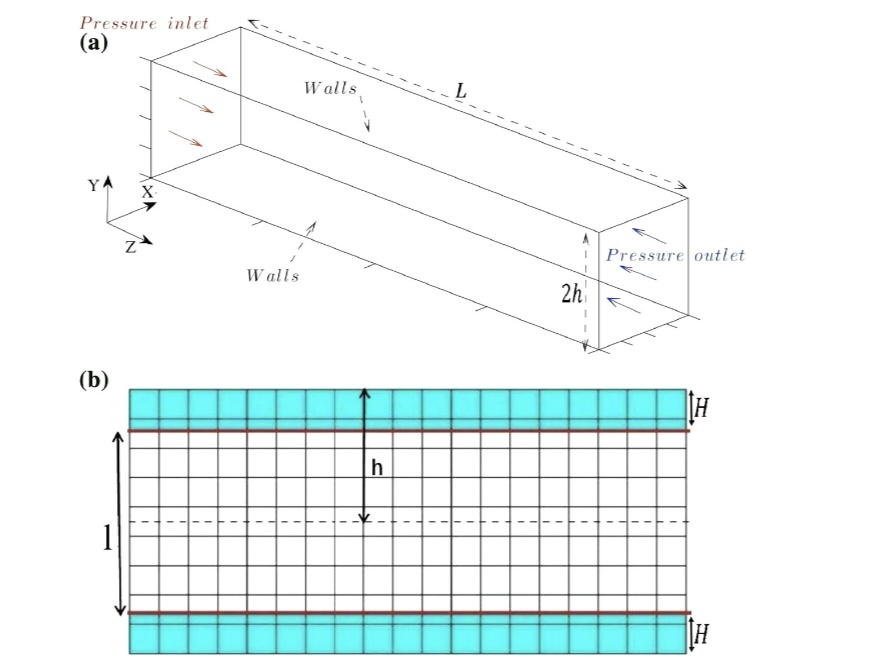
\includegraphics[width=1\linewidth]{IMG_7190.jpeg}
    \caption{Fig. 4 a Computational domain and boundary conditions for fluid flow within a 3D single pore; b longitudinal
view along the flow direction}
    \label{fig:placeholder}
\end{figure}
\FloatBarrier
\begin{equation}
\nabla p = \mu \nabla^2 \mathbf{u}, \tag{61}
\end{equation}

\begin{equation}
\nabla \cdot \mathbf{u} = 0 \tag{62}
\end{equation}

Par conséquent, nous pouvons utiliser une forme simplifiée (Ladd et Verberg 2001) de la fonction de distribution d'équilibre, en négligeant les termes non linéaires dans l'Éq. (9) :

\begin{equation}
f_k^{(eq)} = \omega_k \rho \left[1 + \frac{3(\mathbf{e} \cdot \mathbf{u})}{c^2}\right] \tag{63}
\end{equation}
Cette faible valeur du nombre de Reynolds exclut également les problèmes de compressibilité généralement rencontrés dans les simulations LBM. On peut ainsi considérer une densité du fluide constante, avec :

\begin{equation}
\rho = 1
\end{equation}

(en unités de réseau), pendant l’ensemble des simulations.

Dans un premier temps, les modèles d’écoulement (LBM--FBB, LBM--IBB, IB--LBM1 et IB--LBM2) sont comparés à une solution analytique pour différentes tailles de col de pore.

Ensuite, les modèles couplés de transport réactif et d’écoulement sont évalués par rapport à une solution numérique de référence pour différentes valeurs du nombre de Damköhler.

Il convient de souligner que toutes les simulations sont réalisées sur le maillage initial, sans aucun raffinement du maillage.
\section{Analyse critique des méthodes IB–LB}
Tout d’abord, nous rappelons que la solution analytique d’un écoulement incompressible dans un tube carré infiniment long, défini par :

\begin{equation}
-\frac{l}{2} \leq x,y \leq \frac{l}{2}
\end{equation}

est donnée par l’approximation en série suivante (White, 1991) :
Tout d’abord, nous rappelons que la solution analytique d’un écoulement incompressible dans un tube carré infiniment long, défini par :

\begin{equation}
-\frac{l}{2} \leq x,y \leq \frac{l}{2}
\end{equation}

est donnée par l’approximation en série suivante (White, 1991) :
\begin{equation}
u_z^a(x, y) = \frac{4l^2}{\rho \nu \pi^3} \left( -\frac{dp}{dz} \right) \cdot \sum_{i=1,3,5,\dots}^{\infty} (-1)^{\frac{i-1}{2}} \left[ 1 - \frac{\cosh(i \frac{\pi y}{l})}{\cosh(i \frac{\pi}{2})} \right] \frac{\cos(i \frac{\pi x}{l})}{i^3}. \tag{64}
\end{equation}

où $u_z^a$ est la composante de la vitesse analytique dans la direction de l'écoulement (ici, $z$).

Par conséquent, la vitesse est maximale au centre du tube et peut être approximée par la valeur suivante :

\begin{equation}
V_m \approx 0.5711 \frac{4l^2}{\rho \nu \pi^3} \left( -\frac{dp}{dz} \right). \tag{65}
\end{equation}

Les profils de vitesse résultants selon la direction $y$ sont présentés à la Fig. 5 pour plusieurs valeurs de $l$. La composante de vitesse selon $z$ a été réduite par la vitesse maximale analytique $V_m$ donnée à l'Éq. (65).

La solution LBM–FBB surestime clairement la solution exacte dans tous les cas. Cet écart augmente lorsque l'épaisseur du pore diminue. En effet, bien que l'écart entre la frontière physique et la condition de rebond reste constant, le rapport de cette erreur sur l'épaisseur du pore augmente lorsque $l$ devient plus petit. Dans les pires conditions (c.-à-d. $l = 2.2$), ce rapport, $0.9\Delta x / l$, représente 81 %. De plus, comme montré à l'Éq. (65), la vitesse évolue théoriquement comme une fonction carrée de $l$, ce qui indique que l'erreur relative sur la vitesse est le double de l'erreur relative sur $l$.

À l'inverse, les deux modèles IB–LB ainsi que LB–IBB s'ajustent relativement bien à la solution analytique pour les grands goulots de pore, comme illustré aux Fig. 5a, b. Les méthodes de frontières immergées tendent à sous-estimer la vitesse, tandis que la condition de rebond interpolé tend à la surestimer. Ces trois méthodes montrent une amélioration significative, sauf pour le maillage le plus grossier (Fig. 5d) par rapport à la solution LBM de référence, avec IB–LBM2 démontrant la meilleure précision.

L'écart entre les différentes conditions de traitement des frontières augmente avec la diminution de l'épaisseur du goulot de pore. Lorsque le goulot de pore est trop fin par rapport à la taille du maillage ($l = 2.2$), la méthode IBB se dégrade fortement vers la solution LBM de référence, mais IB–LBM2 conserve une meilleure précision. À ce stade, le nombre de nœuds fluides entre les surfaces solides voisines n'est plus suffisant pour garantir une interpolation précise des distributions de vitesse avec LBM–IBB (Chun et Ladd 2007). Cet inconvénient peut devenir critique pour les écoulements dans des milieux complexes où un colmatage complet des pores se produit.

Un aperçu supplémentaire peut être obtenu par le calcul de l'erreur relative globale :

\begin{equation}
E_i = \sqrt{ \frac{\sum_{x,y} (u_z^a - u_z^i)^2}{\sum_{x,y} (u_z^a)^2} }, \quad i = \text{LBM--FBB, LBM--IBB, IB--LBM1, IB--LBM2} \tag{66}
\end{equation}

où $u_z^a$ est la solution analytique et $u_z^i$ est la solution numérique calculée par la méthode LBM ou IB–LB. Les résultats sont regroupés dans le Tableau 1 pour les différentes simulations et à la Fig. 5e.

Les différents modèles sont également comparés en termes d'efficacité. La performance des simulations est mesurée en temps CPU, indiqué pour chaque calcul dans le Tableau 1 et à la Fig. 5f. Toutes les simulations ont été réalisées en double précision sur une station de travail dual Xeon 2.4 GHz. Le temps de calcul dépend du nombre de nœuds du réseau, mais aussi du nombre d'itérations nécessaires pour atteindre l'état stationnaire. Ces deux facteurs produisent des effets opposés. Lorsque les goulots de pore deviennent plus étroits, le nombre de nœuds diminue, entraînant une réduction du temps de calcul, mais les modèles nécessitent plus d'itérations pour converger. Comme observé avec les profils de vitesse, le schéma interpolé montre une erreur significativement plus faible que le cas de référence, avec une exception notable lorsque $l = 2.2$, ainsi qu'une légère augmentation du temps de calcul (environ 20 %). IB–LBM2 montre une meilleure précision, cependant avec une augmentation significative du temps de calcul.
\begin{figure}[H]
    \centering
    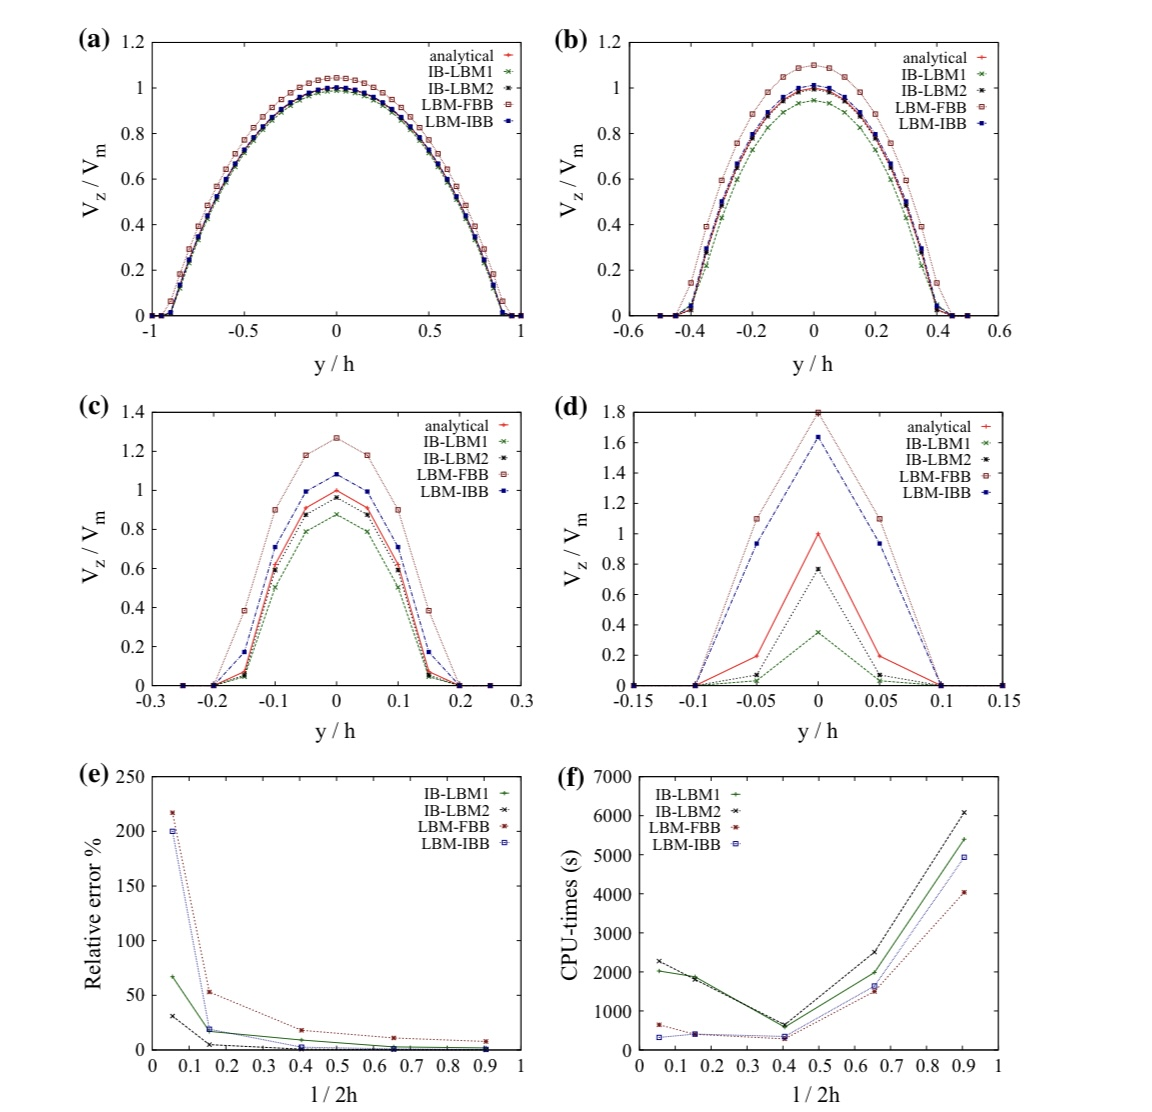
\includegraphics[width=1\linewidth]{IMG_7195.jpeg}
    \caption{Fig. 5 Comparaison des profils de vitesse selon l’axe z pour les méthodes LBM–FBB, LBM–IBB et IB–LBM avec la solution analytique pour différentes valeurs de l :

a) l = 36.2 ;
b) l = 16.2 ;
c) l = 6.2 ;
d) l = 2.2 ;
e) erreur relative globale obtenue par les méthodes LBM–FBB, LBM–IBB et les deux méthodes IB–LBM ;
f) temps de calcul CPU pour chaque méthode.}
    \label{fig:placeholder}
\end{figure}
\FloatBarrier
Le coût de calcul peut atteindre jusqu’à quatre fois celui du cas de référence. La méthode IB--LBM1 présente des temps de calcul comparables à ceux de IB--LBM2, mais avec une précision plus faible.

Deux résultats principaux ressortent de ces calculs :

\begin{itemize}
\item Pour un maillage fin ($l = 36.2$), aucune différence marquante n’est observée entre les modèles ; l’erreur ne dépasse pas $7.2\%$ avec la méthode LBM--FBB.

\item Lorsque le pore se rétrécit (ou lorsque le maillage devient plus grossier), l’importance des schémas interpolés et des méthodes de frontières immergées apparaît clairement pour les calculs à l’échelle du pore. La précision des schémas interpolés se dégrade fortement sur des maillages très grossiers.
\end{itemize}

Sur un maillage grossier (par exemple $l = 6.2$), l’erreur relative obtenue avec IB--LBM2 est dix fois plus faible que celle de la méthode classique LBM--FBB, et quatre fois plus faible que celles de IB--LBM1 et LBM--IBB.
\begin{figure}[H]
    \centering
    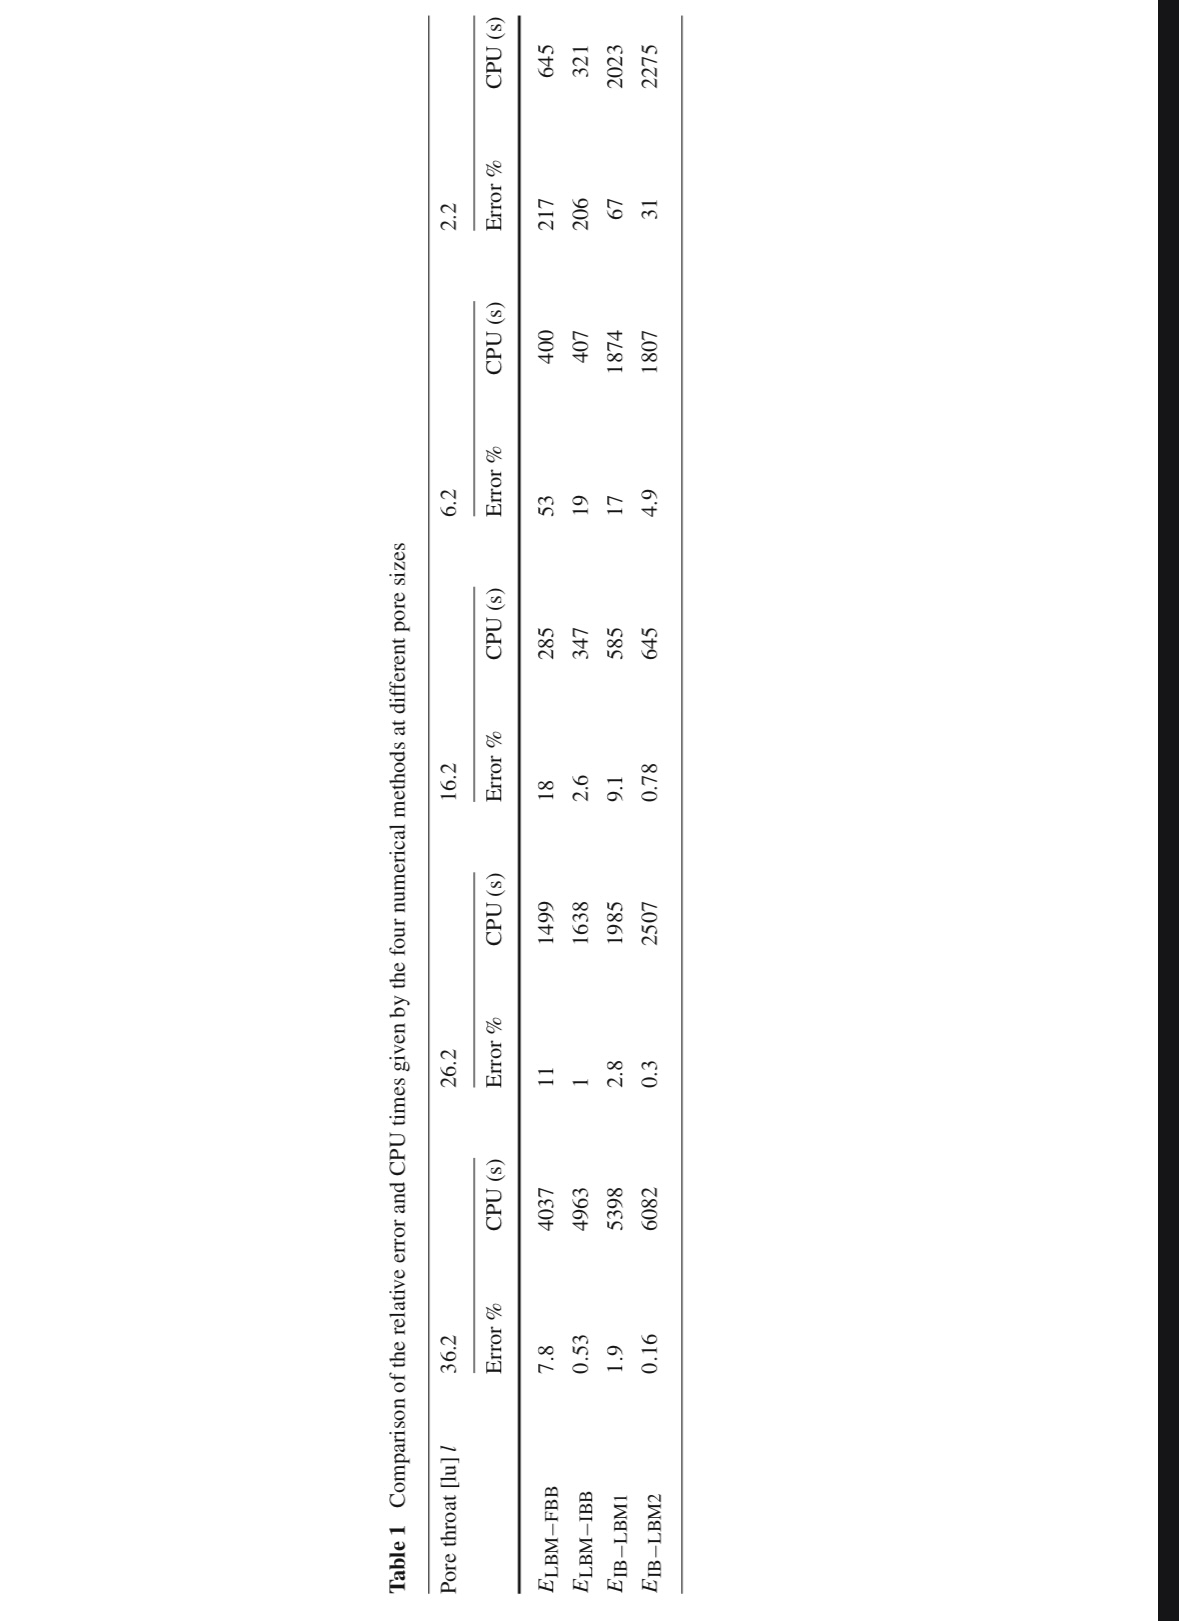
\includegraphics[width=1\linewidth]{IMG_7196.jpeg}

    \label{fig:placeholder}
\end{figure}
\FloatBarrier
\begin{itemize}
\item Si l’on considère une valeur seuil arbitraire de $10\%$ pour la précision des simulations, la Fig.~5e montre que la taille du pore peut diminuer de $90\%$ avant qu’un raffinement du maillage ne soit nécessaire avec la méthode IB--LBM2, contre $75\%$ pour IB--LBM1 et à peine $30\%$ pour la méthode LBM classique.

\item Dans le même ordre d’idées, pour une taille de pore donnée, un maillage plus grossier peut être utilisé avec IB--LBM2 par rapport à une simulation classique par la méthode de Boltzmann sur réseau, sans perte de précision.

\item Ce gain peut devenir très significatif en temps de calcul, particulièrement en trois dimensions. Cette amélioration compense probablement le surcoût lié à la complexité du modèle.
\end{itemize}

Par exemple, une analyse croisée des Fig.~5e et 5f indique que le temps de calcul nécessaire pour obtenir une erreur de $1\%$ avec LBM--IBB ($l = 26.2$) est supérieur à trois fois celui requis avec IB--LBM2 (où $l = 16.2$ est suffisant).
\section{Discussion sur le transport réactif}
À ce stade, nous considérons le transport des espèces réactives à travers le pore unique, tel que décrit par les équations (36)--(41). Le domaine de calcul reste identique (Fig.~4). Le soluté peut diffuser à l’intérieur du matériau imperméable de $\Omega_r$, où il est consommé par réaction chimique.

Afin d’étudier l’impact de l’évolution temporelle de la géométrie sur la qualité du maillage et la précision de la solution, nous faisons varier la taille du maillage plutôt que l’épaisseur des parois, contrairement à l’étude précédente. Ainsi, des conditions similaires (mêmes longueurs caractéristiques, même nombre de Péclet) sont conservées pour toutes les simulations afin de permettre une comparaison pertinente entre les différents modèles de transport.

L’épaisseur de la paroi réactive est maintenue constante, avec :

\begin{equation}
\frac{H}{h}=0.172
\end{equation}

ou encore :

\begin{equation}
\frac{l}{h}=0.656
\end{equation}

Dans un objectif de comparaison, le même champ de vitesse est conservé pour toutes les simulations. Le maillage cartésien utilisé par la méthode des volumes finis coïncide avec le maillage du réseau, de sorte que les nœuds de vitesse et de concentration se superposent.

Nous nous limitons à l’étude des profils de concentration en régime stationnaire. En raison de la dépendance de la vitesse du front à la précision du modèle, les profils transitoires ne seraient pas cohérents et leur comparaison n’aurait pas de sens.

Le cas étudié est le suivant : le soluté est injecté par la face d’entrée à concentration constante $C_0$. Les coefficients de diffusion dans $\Omega_f$ et $\Omega_r$ sont différents, avec :

\begin{equation}
\frac{D_r}{D_f}=0.25
\end{equation}

Les longueurs caractéristiques utilisées pour le calcul des nombres de Péclet et de Damköhler (Eq.~60) sont respectivement $l$ et $H$. Ainsi, une valeur constante est imposée :

\begin{equation}
Pe=6.5
\end{equation}

pour l’ensemble des simulations.

Deux valeurs du nombre de Damköhler sont considérées :

\begin{equation}
Da=1.2
\end{equation}

et

\begin{equation}
Da=12
\end{equation}

ainsi que deux tailles de maillage :

\begin{equation}
17 \times 17 \times 17
\end{equation}

et

\begin{equation}
35 \times 35 \times 35
\end{equation}

Cette plage de valeurs de $Da$ correspond à des conditions de réaction faibles à modérées, typiquement rencontrées dans les applications souterraines.

La solution de référence pour cette géométrie est obtenue à partir d’une simulation raffinée utilisant LBM pour l’écoulement et la méthode des volumes finis pour le transport de concentration.

Comme précédemment, le maillage de calcul et la frontière physique ne coïncident pas, avec un décalage constant de :

\begin{equation}
0.745\Delta x
\end{equation}

pour le maillage $17 \times 17 \times 17$, et :

\begin{equation}
0.65\Delta x
\end{equation}

pour le maillage $35 \times 35 \times 35$.

Trois simulations distinctes sont réalisées sur chacun des maillages.

La première consiste en une simulation LBM avec condition classique de rebond complet (\textit{full-way bounce-back}) pour l’écoulement et méthode des volumes finis pour le transport du soluté, notée LBM--FBB--FV. Elle sert de référence comparative afin d’illustrer l’impact de la dégradation du maillage sur la précision, en l’absence de méthode non conforme aux frontières.

Les deux autres simulations diffèrent par la méthode de transport utilisée :

\begin{itemize}
\item méthode Volume of Fluid (VOF),
\item méthode de reconstruction (REC).
\end{itemize}

Conformément aux résultats de la section 4.1, la méthode de frontière immergée retenue pour le calcul de l’écoulement est la plus précise, à savoir :

\begin{equation}
IB\text{--}LBM2
\end{equation}

La comparaison des profils de concentration au centre du domaine est présentée dans les Fig.~6 et 7 pour les deux tailles de maillage et les deux valeurs de $Da$.

L’erreur relative sur le flux massique prédite par les différentes méthodes est extraite de ces figures et comparée dans les Tableaux~2.

\section{Limites et hypothèses de l’étude}
Quasi-stationnarité, géométrie simplifiée.

% -------------------------
% CHAPITRE 7 — CONCLUSION
% -------------------------

\chapter{Conclusion générale et perspectives}

\section{Principales contributions}
\section{Perspectives scientifiques}
\begin{itemize}
    \item Simulation couplée dynamique (temps réel)
    \item Extension MRT
    \item Application au bio-clogging ou au stockage de gaz
\end{itemize}

% -------------------------
% ANNEXES
% -------------------------

\appendix
\chapter{Annexes}
\section{Paramètres numériques détaillés}
\section{Algorithmes IB–LB}
\section{Figures supplémentaires}

% -------------------------
% BIBLIOGRAPHIE
% -------------------------

\begin{thebibliography}{99}
\bibitem{articleIBLB}
M. Benioug et al., \textit{Numerical Efficiency Assessment of IB–LB Method for 3D Pore-Scale Modeling of Flow and Transport}.
\end{thebibliography}

\end{document}

